\documentclass[11pt,onside]{article}
\usepackage[a4paper]{geometry}
\usepackage[utf8]{inputenc}
\usepackage[english]{babel}
\usepackage{lipsum}
\usepackage{bm}
\usepackage{upgreek}
\usepackage[noend]{algpseudocode}
\usepackage{algorithm}
\usepackage{amsmath}
\usepackage{float}
\usepackage{graphicx} % Required for including images

\usepackage{algpseudocode}
% mathtools for: Aboxed (put box on last equation in align envirenment)
\usepackage{microtype} %improves the spacing between words and letters

%% COLOR DEFINITIONS

\usepackage[svgnames]{xcolor} % Enabling mixing colors and color's call by 'svgnames'

\definecolor{MyColor1}{rgb}{0.2,0.4,0.6} %mix personal color
\newcommand{\textb}{\color{Black} \usefont{OT1}{lmss}{m}{n}}
\newcommand{\blue}{\color{MyColor1} \usefont{OT1}{lmss}{m}{n}}
\newcommand{\blueb}{\color{MyColor1} \usefont{OT1}{lmss}{b}{n}}
\newcommand{\red}{\color{LightCoral} \usefont{OT1}{lmss}{m}{n}}
\newcommand{\green}{\color{Turquoise} \usefont{OT1}{lmss}{m}{n}}

\DeclareMathOperator{\trace}{trace}
\DeclareMathOperator{\diag}{diag}

%% FONTS AND COLORS

%    SECTIONS

\usepackage{titlesec}
\usepackage{sectsty}
%%%%%%%%%%%%%%%%%%%%%%%%
%set section/subsections HEADINGS font and color
\sectionfont{\color{MyColor1}}  % sets colour of sections
\subsectionfont{\color{MyColor1}}  % sets colour of sections

%set section enumerator to arabic number (see footnotes markings alternatives)
\renewcommand\thesection{\arabic{section}.} %define sections numbering
\renewcommand\thesubsection{\thesection\arabic{subsection}} %subsec.num.

%define new section style
\newcommand{\mysection}{
\titleformat{\section} [runin] {\usefont{OT1}{lmss}{b}{n}\color{MyColor1}} 
{\thesection} {3pt} {} } 


%	CAPTIONS
\usepackage{caption}
\usepackage{subcaption}
%%%%%%%%%%%%%%%%%%%%%%%%
\captionsetup[figure*]{labelfont={color=Turquoise}}


%		!!!EQUATION (ARRAY) --> USING ALIGN INSTEAD
%using amsmath package to redefine eq. numeration (1.1, 1.2, ...) 
\renewcommand{\theequation}{\thesection\arabic{equation}}



\makeatletter
\let\reftagform@=\tagform@
\def\tagform@#1{\maketag@@@{(\ignorespaces\textcolor{red}{#1}\unskip\@@italiccorr)}}
\renewcommand{\eqref}[1]{\textup{\reftagform@{\ref{#1}}}}
\makeatother
\usepackage{hyperref}
\hypersetup{colorlinks=true}

% For labeling top of page on every page but first one:
\usepackage{fancyhdr}

% PREPARE TITLE:
\title{\blue Adversarial Robustness-toolbox \\
\blueb Generate Counter Examples}
\author{Fast Gradient Method, Basic Iterative Method, Deep Fool}

\renewcommand{\rmdefault}{phv} % Arial Font
\renewcommand{\sfdefault}{phv} % Arial Font

\pagestyle{fancy}
\fancyhead{}
\fancyhead[CO,CE]{{\small{{\bf{Adversarial Robustness-toolbox}} - Counter Examples}}}
 

\begin{document}
\maketitle


\section{Label Counts}

\begin{figure*}[h]
\centering
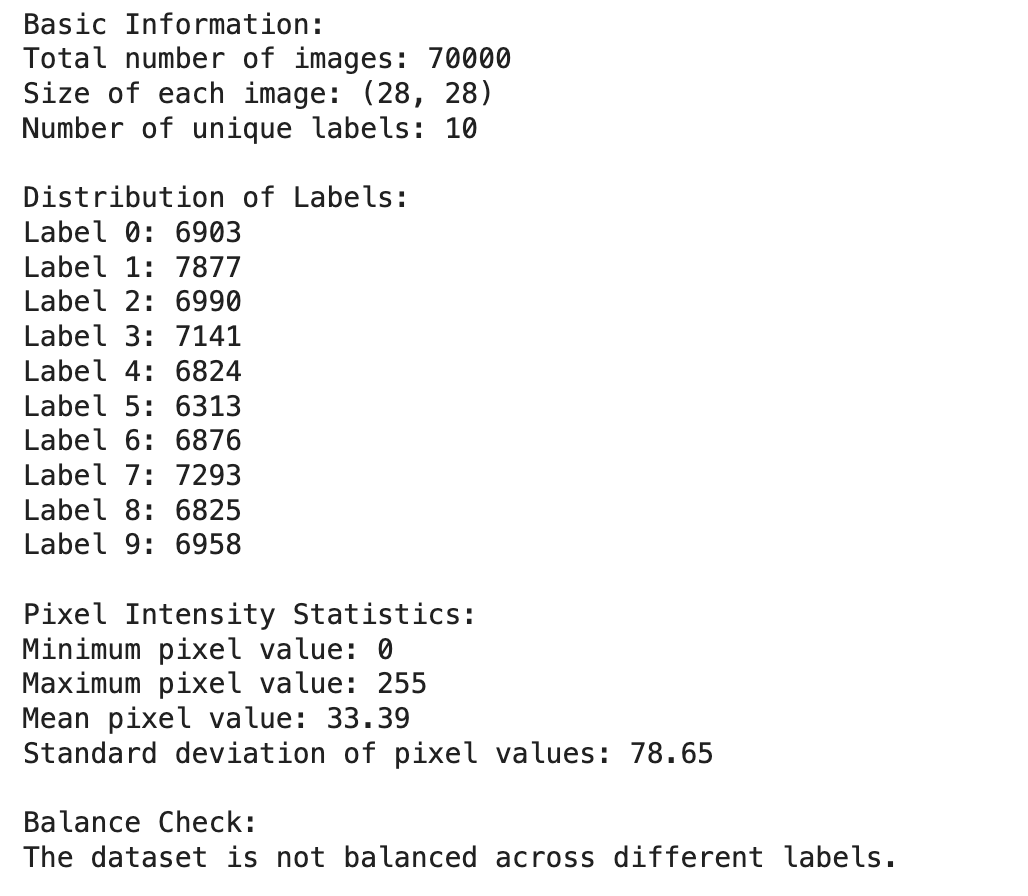
\includegraphics[width=0.8\textwidth]{V2_images/basic_info.png}
\caption{Basic Information of Dataset}
\label{fig:Basic Information of Dataset}
\end{figure*}



\begin{algorithm}[H]
\caption{Evaluation of a Pre-trained Model on MNIST Dataset}
\begin{algorithmic}[1]
\Require Pre-trained model path $\mathcal{P}_{\text{model}}$, MNIST dataset
\Ensure Test accuracy, Correct examples and labels saved

\Function{LoadModel}{$\mathcal{P}_{\text{model}}$}
    \State $\mathcal{M} \gets$ load model from $\mathcal{P}_{\text{model}}$
    \State \Return $\mathcal{M}$
\EndFunction

\Function{LoadMNISTData}{}
    \State $(\mathcal{X}_{\text{train}}, \mathcal{Y}_{\text{train}}), (\mathcal{X}_{\text{test}}, \mathcal{Y}_{\text{test}}) \gets$ MNIST data
    \State \Return $(\mathcal{X}_{\text{train}}, \mathcal{Y}_{\text{train}}), (\mathcal{X}_{\text{test}}, \mathcal{Y}_{\text{test}})$
\EndFunction

\Function{PreprocessData}{$\mathcal{X}$}
    \State $\mathcal{X} \gets$ reshape and normalize $\mathcal{X}$
    \State \Return $\mathcal{X}$
\EndFunction

\Function{OneHotEncode}{$\mathcal{Y}$}
    \State $\mathcal{Y}_{\text{encoded}} \gets$ one-hot encode $\mathcal{Y}$
    \State \Return $\mathcal{Y}_{\text{encoded}}$
\EndFunction

\Function{EvaluateModel}{$\mathcal{M}$, $\mathcal{X}_{\text{test}}$, $\mathcal{Y}_{\text{test}}$}
    \State $\mathcal{P} \gets$ model predictions for $\mathcal{X}_{\text{test}}$
    \State $\mathcal{L}, \mathcal{A} \gets$ evaluate $\mathcal{M}$ on $\mathcal{X}_{\text{test}}$ and $\mathcal{Y}_{\text{test}}$
    \State \Return $\mathcal{P}$, $\mathcal{L}$, $\mathcal{A}$
\EndFunction

\Function{SaveCorrect}{$\mathcal{X}_{\text{test}}$, $\mathcal{Y}_{\text{test}}$, $\mathcal{P}$}
    \State $\mathcal{I}_{\text{correct}} \gets$ indices where $\mathcal{P}$ equals $\mathcal{Y}_{\text{test}}$
    \State $\mathcal{X}_{\text{correct}} \gets$ examples from $\mathcal{X}_{\text{test}}$ at $\mathcal{I}_{\text{correct}}$
    \State $\mathcal{Y}_{\text{correct}} \gets$ labels from $\mathcal{Y}_{\text{test}}$ at $\mathcal{I}_{\text{correct}}$
    \State Save $\mathcal{X}_{\text{correct}}$ and $\mathcal{Y}_{\text{correct}}$ to disk
\EndFunction

\State $\mathcal{M} \gets$ \Call{LoadModel}{$\mathcal{P}_{\text{model}}$}
\State $(\mathcal{X}_{\text{train}}, \mathcal{Y}_{\text{train}}), (\mathcal{X}_{\text{test}}, \mathcal{Y}_{\text{test}}) \gets$ \Call{LoadMNISTData}{}
\State $\mathcal{X}_{\text{train}} \gets$ \Call{PreprocessData}{$\mathcal{X}_{\text{train}}$}
\State $\mathcal{X}_{\text{test}} \gets$ \Call{PreprocessData}{$\mathcal{X}_{\text{test}}$}
\State $\mathcal{Y}_{\text{train}} \gets$ \Call{OneHotEncode}{$\mathcal{Y}_{\text{train}}$}
\State $\mathcal{Y}_{\text{test}} \gets$ \Call{OneHotEncode}{$\mathcal{Y}_{\text{test}}$}
\State $\mathcal{P}$, $\mathcal{L}$, $\mathcal{A} \gets$ \Call{EvaluateModel}{$\mathcal{M}$, $\mathcal{X}_{\text{test}}$, $\mathcal{Y}_{\text{test}}$}
\State Print $\mathcal{A}$ as test accuracy
\State \Call{SaveCorrect}{$\mathcal{X}_{\text{test}}$, $\mathcal{Y}_{\text{test}}$, $\mathcal{P}$}

\end{algorithmic}
\end{algorithm}



\begin{figure*}[h]
\centering
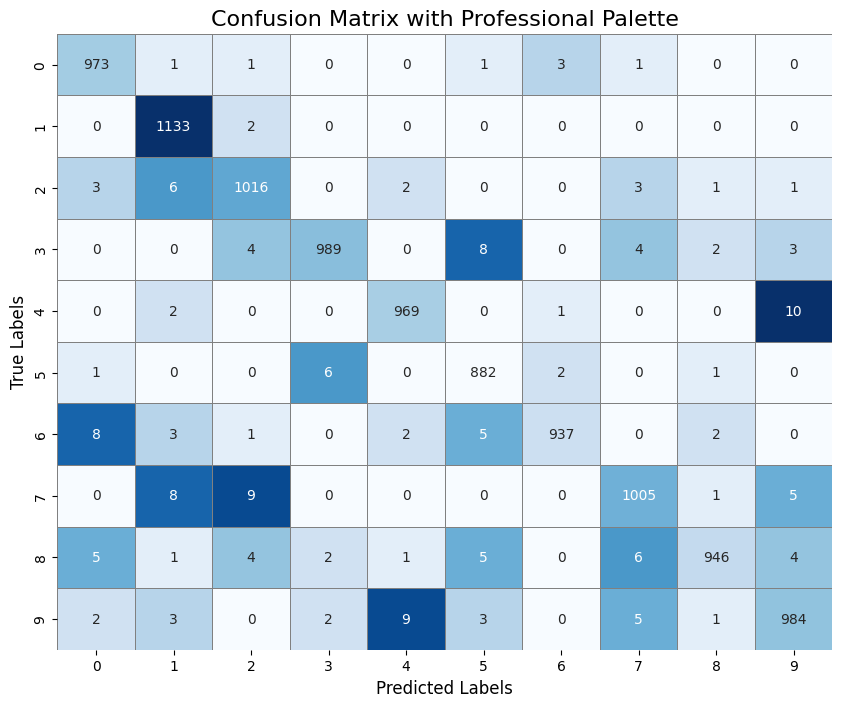
\includegraphics[width=0.8\textwidth]{V2_images/model.png}
\caption{CM FSGM (Test accuracy: 0.983) }
\label{fig:FSGM}
\end{figure*}


\begin{table}[h]
\centering
\caption{Label counts}
\begin{tabular}{|l|l|l|l|l|l|}
\hline
               & \textbf{\begin{tabular}[c]{@{}l@{}}Total \\ MNIST\end{tabular}} & \textbf{\begin{tabular}[c]{@{}l@{}}Training \\ Set\end{tabular}} & \textbf{\begin{tabular}[c]{@{}l@{}}Test \\ Set\end{tabular}} & \textbf{\begin{tabular}[c]{@{}l@{}}Predict \\ Labels\end{tabular}} & \textbf{\begin{tabular}[c]{@{}l@{}}Correct \\ Labels\end{tabular}} \\ \hline
\textbf{0}     & 6903                                                            & 5923                                                             & 980                                                          & 992                                                                & 973                                                                \\ \hline
\textbf{1}     & 7877                                                            & 6742                                                             & 1135                                                         & 1157                                                               & 1130                                                               \\ \hline
\textbf{2}     & 6990                                                            & 5958                                                             & 1032                                                         & 1037                                                               & 1015                                                               \\ \hline
\textbf{3}     & 7141                                                            & 6131                                                             & 1010                                                         & 999                                                                & 993                                                                \\ \hline
\textbf{4}     & 6824                                                            & 5842                                                             & 982                                                          & 983                                                                & 968                                                                \\ \hline
\textbf{5}     & 6313                                                            & 5421                                                             & 892                                                          & 904                                                                & 882                                                                \\ \hline
\textbf{6}     & 6876                                                            & 5918                                                             & 958                                                          & 943                                                                & 942                                                                \\ \hline
\textbf{7}     & 7293                                                            & 6265                                                             & 1028                                                         & 1024                                                               & 1007                                                               \\ \hline
\textbf{8}     & 6825                                                            & 5851                                                             & 974                                                          & 954                                                                & 965                                                                \\ \hline
\textbf{9}     & 6958                                                            & 5949                                                             & 1009                                                         & 1007                                                               & 990                                                                \\ \hline
\textbf{Total} & \textbf{70000}                                                  & \textbf{60000}                                                   & \textbf{10000}                                               & \textbf{10000}                                                     & \textbf{9865}                                                      \\ \hline
\end{tabular}

\end{table}

\clearpage % This will ensure that the title page is cleared before your sections start

\section{FSGM Without True Labels}

\begin{algorithm}[H]
\caption{Adversarial Example Generation and Analysis}
\begin{algorithmic}[1]
\State $\textbf{Input:}$ classifier, correct\_examples, correct\_labels
\State $\textbf{Output:}$ results\_df, confusion matrices
\State $\text{eps\_range} \gets [0.01, 0.02, \ldots, 0.6]$
\State $\text{results\_df} \gets \text{DataFrame with columns ['eps', 'total\_correct', 'total\_adv', 'correct\_adv\_counts']}$
\For{$\text{eps} \in \text{eps\_range}$}
    \State $\text{attack} \gets \text{FastGradientMethod}(\text{classifier}, \text{eps})$
    \State $\text{x\_adv} \gets \text{attack.generate}(\text{x=correct\_examples})$
    \State $\text{y\_adv} \gets \text{argmax}(\text{classifier.predict}(\text{x\_adv}), \text{axis}=1)$
    \State $\text{adv\_counts} \gets \text{count\_unique}(\text{y\_adv})$
    \State $\text{cm} \gets \text{confusion\_matrix}(\text{correct\_labels}, \text{y\_adv})$
    \State $\text{Save heatmap of cm to file with filename based on eps}$
    \State $\text{results\_df.append}(\{\text{'eps'}: \text{eps}, \text{'total\_correct'}: \text{length(correct\_labels)}, \text{'total\_adv'}: \text{length(y\_adv)}, \text{'correct\_adv\_counts'}: \text{adv\_counts}\})$
\EndFor
\State $\text{results\_df.to\_csv}(\text{'/content/drive/MyDrive/ColabNotebooks/adv\_results\_labels.csv'})$
\end{algorithmic}
\end{algorithm}


\begin{figure*}[h]
  \centering
  \begin{subfigure}[b]{0.49\textwidth}
    \centering
    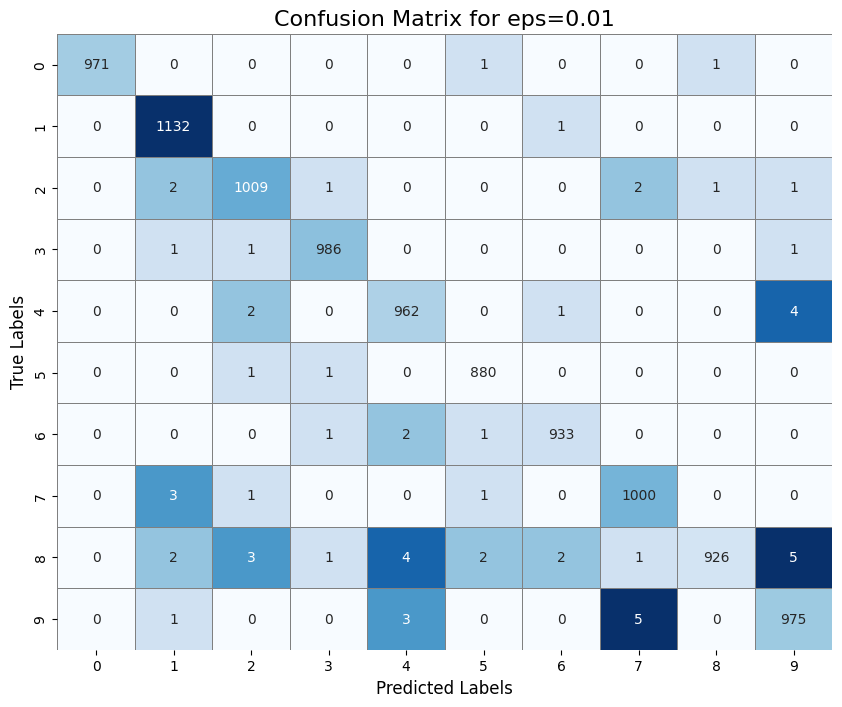
\includegraphics[width=\textwidth]{V2_images/confusion_matrix_eps_0.01.png}
    \caption{confusion matrix 0.01}
    \label{fig:image1}
  \end{subfigure}
  \hfill
  \begin{subfigure}[b]{0.49\textwidth}
    \centering
    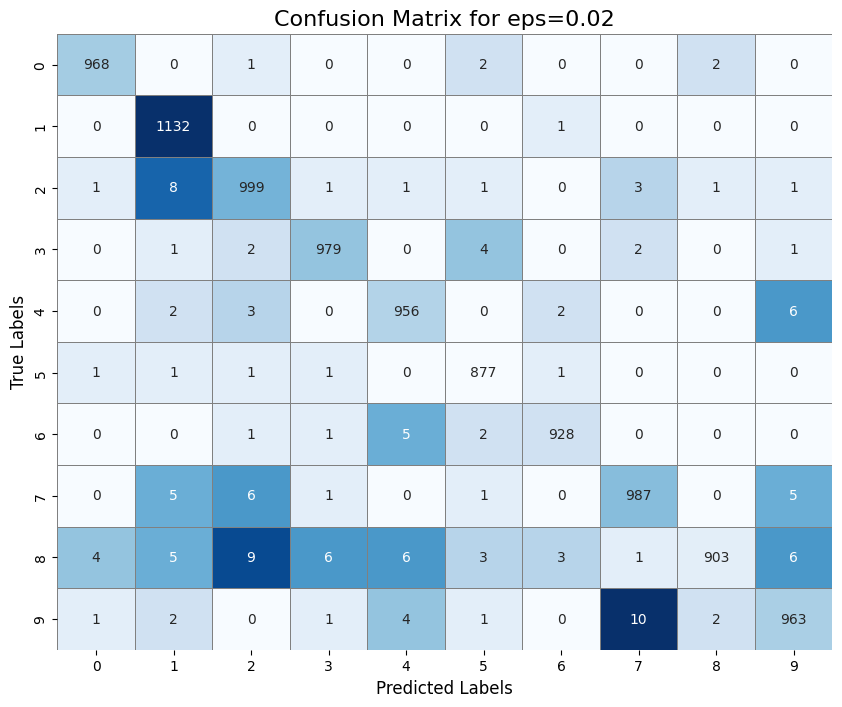
\includegraphics[width=\textwidth]{V2_images/confusion_matrix_eps_0.02.png}
    \caption{confusion matrix 0.02}
    \label{fig:image2}
  \end{subfigure}

  \label{fig:images}
\end{figure*}


\begin{figure*}[h]
  \centering
  \begin{subfigure}[b]{0.49\textwidth}
    \centering
    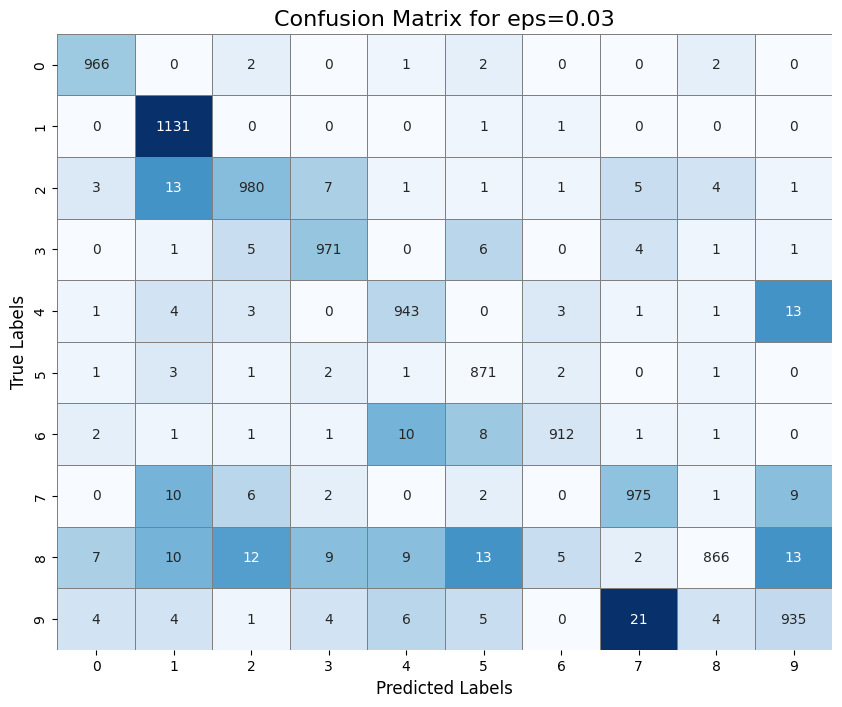
\includegraphics[width=\textwidth]{V2_images/confusion_matrix_eps_0.03.png}
    \caption{confusion matrix 0.03}
    \label{fig:image1}
  \end{subfigure}
  \hfill
  \begin{subfigure}[b]{0.49\textwidth}
    \centering
    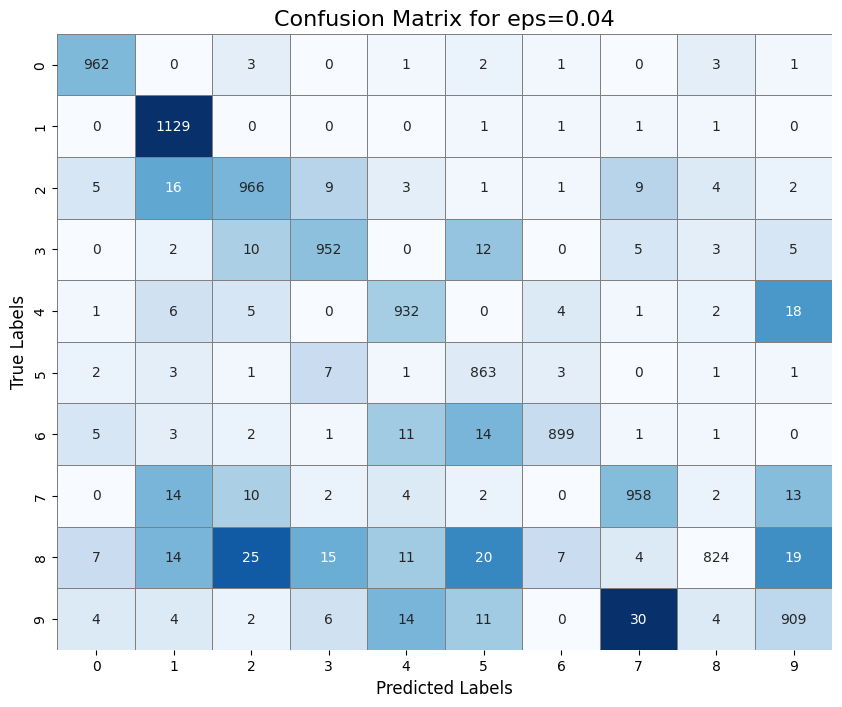
\includegraphics[width=\textwidth]{V2_images/confusion_matrix_eps_0.04.png}
    \caption{confusion matrix 0.04}
    \label{fig:image2}
  \end{subfigure}

  \label{fig:images}
\end{figure*}


\begin{figure*}[h]
  \centering
  \begin{subfigure}[b]{0.49\textwidth}
    \centering
    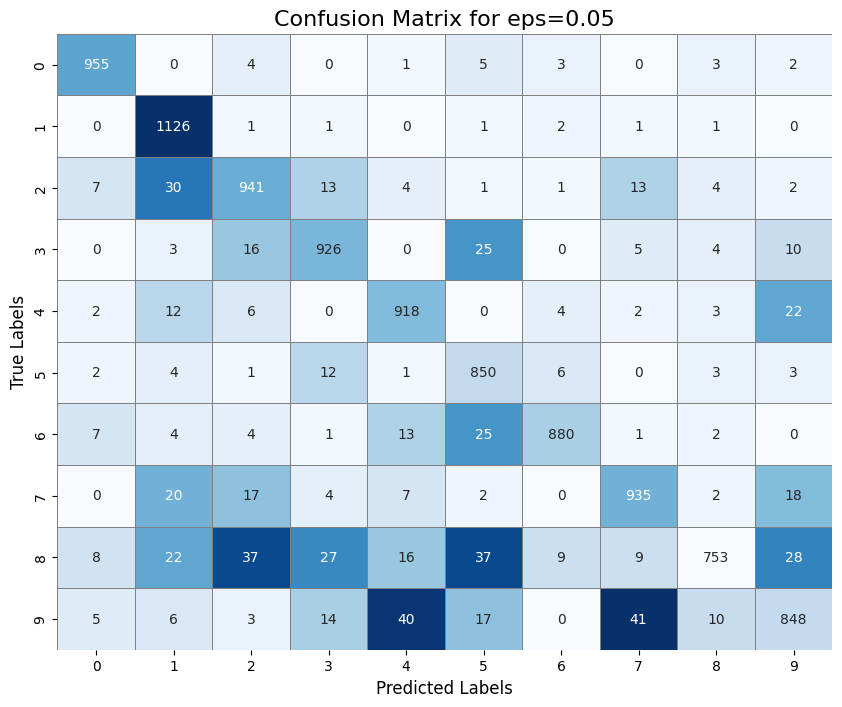
\includegraphics[width=\textwidth]{V2_images/confusion_matrix_eps_0.05.png}
    \caption{confusion matrix 0.05}
    \label{fig:image1}
  \end{subfigure}
  \hfill
  \begin{subfigure}[b]{0.49\textwidth}
    \centering
    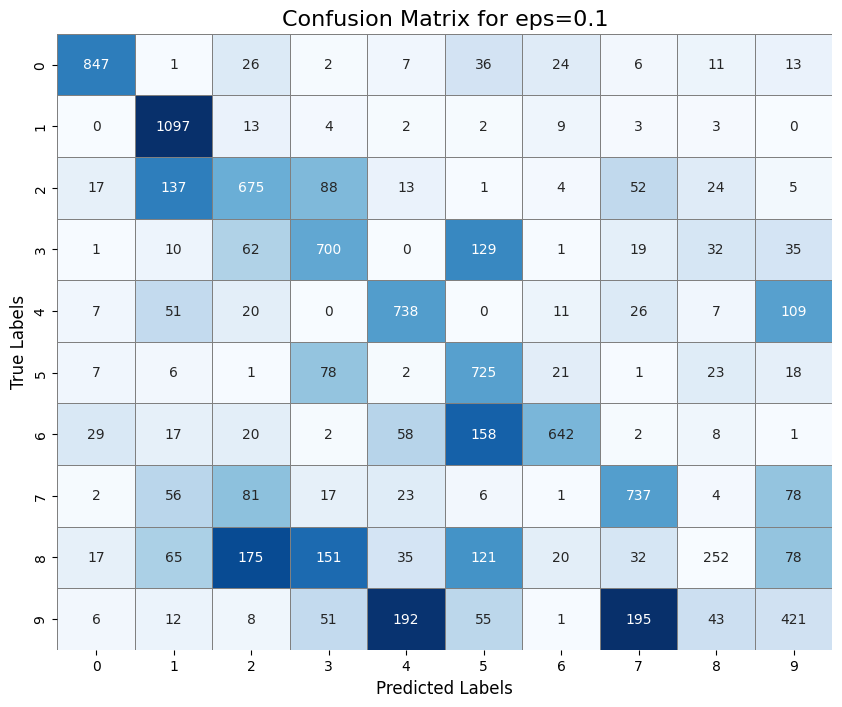
\includegraphics[width=\textwidth]{V2_images/confusion_matrix_eps_0.1.png}
    \caption{confusion matrix 0.1}
    \label{fig:image2}
  \end{subfigure}

  \label{fig:images}
\end{figure*}

\begin{figure*}[h]
  \centering
  \begin{subfigure}[b]{0.49\textwidth}
    \centering
    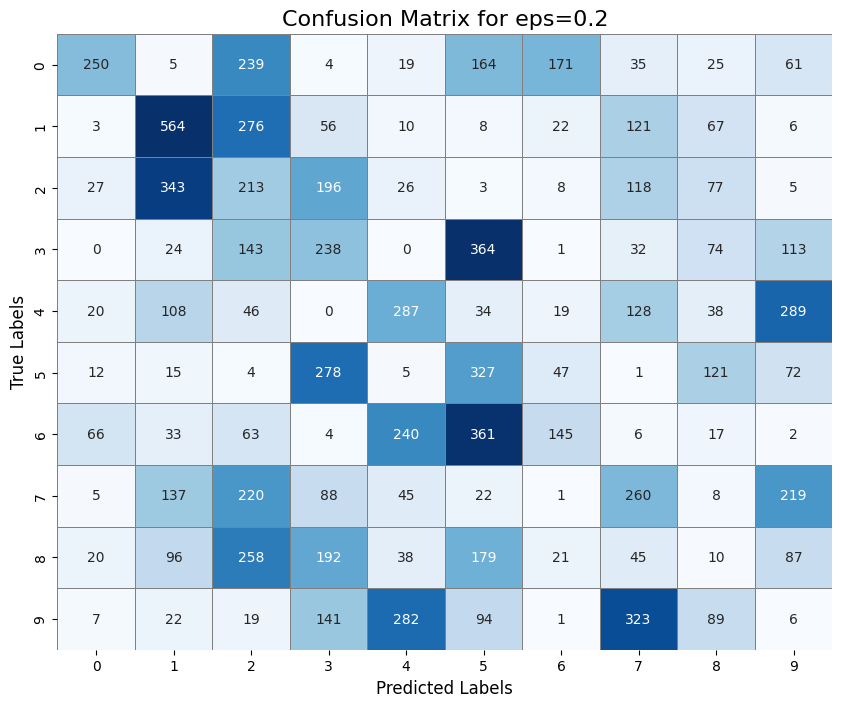
\includegraphics[width=\textwidth]{V2_images/confusion_matrix_eps_0.2.png}
    \caption{confusion matrix 0.2}
    \label{fig:image1}
  \end{subfigure}
  \hfill
  \begin{subfigure}[b]{0.49\textwidth}
    \centering
    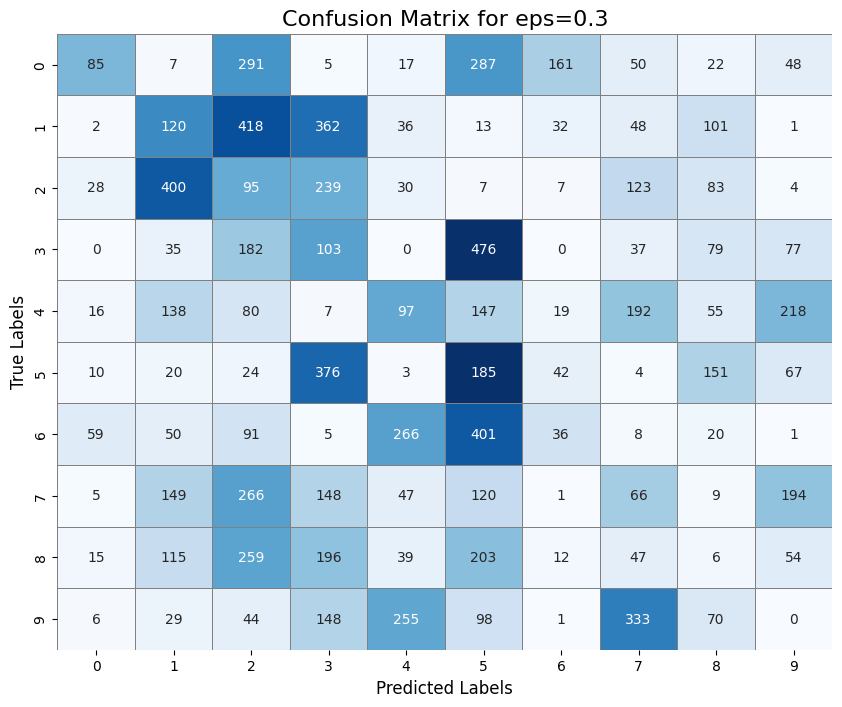
\includegraphics[width=\textwidth]{V2_images/confusion_matrix_eps_0.3.png}
    \caption{confusion matrix 0.3}
    \label{fig:image2}
  \end{subfigure}
 
  \label{fig:images}
\end{figure*}


\begin{figure*}[h]
  \centering
  \begin{subfigure}[b]{0.49\textwidth}
    \centering
    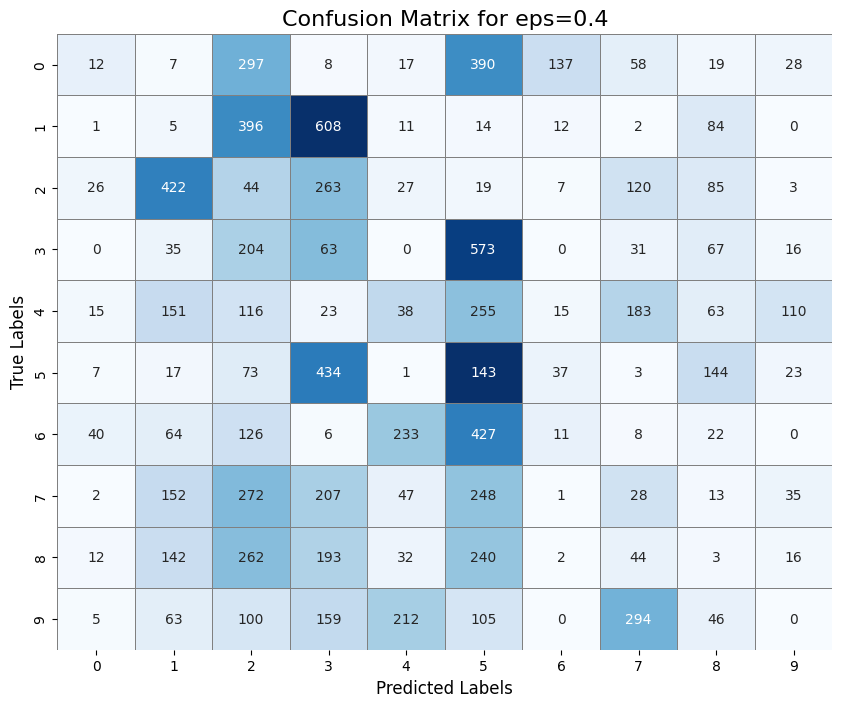
\includegraphics[width=\textwidth]{V2_images/confusion_matrix_eps_0.4.png}
    \caption{confusion matrix 0.4}
    \label{fig:image1}
  \end{subfigure}
  \hfill
  \begin{subfigure}[b]{0.49\textwidth}
    \centering
    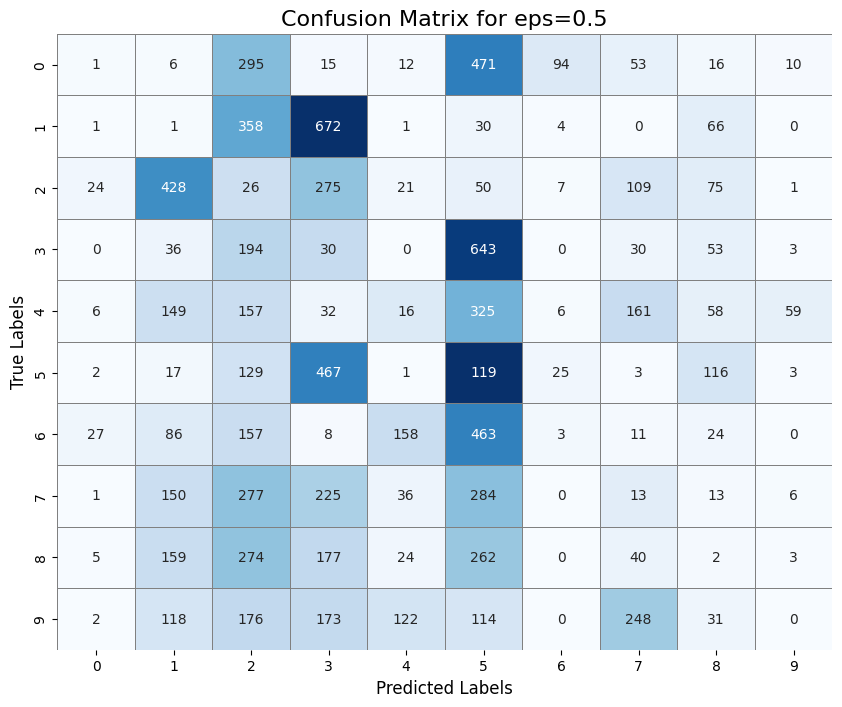
\includegraphics[width=\textwidth]{V2_images/confusion_matrix_eps_0.5.png}
    \caption{confusion matrix 0.5}
    \label{fig:image2}
  \end{subfigure}

  \label{fig:images}
\end{figure*}

\begin{figure*}[h]
  \centering
  \begin{subfigure}[b]{0.49\textwidth}
    \centering
    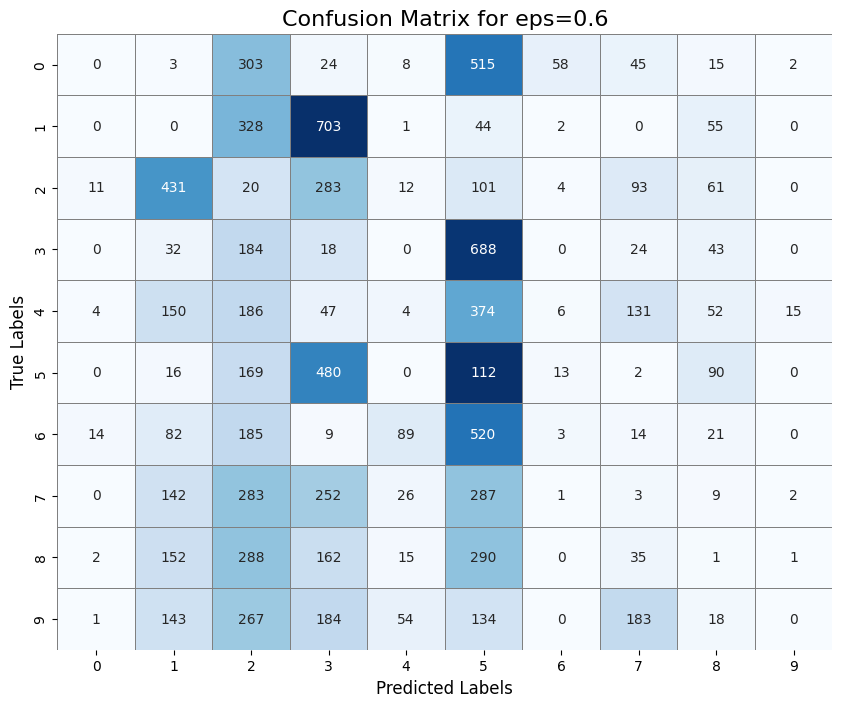
\includegraphics[width=\textwidth]{V2_images/confusion_matrix_eps_0.6.png}
    \caption{confusion matrix 0.6}
    \label{fig:image1}
  \end{subfigure}
 
\end{figure*}
\clearpage % This will ensure that the title page is cleared before your sections start


\section{FSGM With True Labels}

\begin{algorithm}[H]
\caption{Adversarial Example Generation and Analysis}
\begin{algorithmic}[1]
\State $\textbf{Input:}$ classifier, correct\_examples, correct\_labels
\State $\textbf{Output:}$ results\_df, confusion matrices
\State $\text{eps\_range} \gets [0.01, 0.02, \ldots, 0.6]$
\State $\text{results\_df} \gets \text{DataFrame with columns ['eps', 'total\_correct', 'total\_adv', 'correct\_adv\_counts']}$
\For{$\text{eps} \in \text{eps\_range}$}
    \State $\text{attack} \gets \text{FastGradientMethod}(\text{classifier}, \text{eps})$
    \State $\text{x\_adv} \gets \text{attack.generate}(\text{x=correct\_examples, y=correct\_labels})$
    \State $\text{y\_adv} \gets \text{argmax}(\text{classifier.predict}(\text{x\_adv}), \text{axis}=1)$
    \State $\text{adv\_counts} \gets \text{count\_unique}(\text{y\_adv})$
    \State $\text{cm} \gets \text{confusion\_matrix}(\text{correct\_labels}, \text{y\_adv})$
    \State $\text{Save heatmap of cm to file with filename based on eps}$
    \State $\text{results\_df.append}(\{\text{'eps'}: \text{eps}, \text{'total\_correct'}: \text{length(correct\_labels)}, \text{'total\_adv'}: \text{length(y\_adv)}, \text{'correct\_adv\_counts'}: \text{adv\_counts}\})$
\EndFor
\State $\text{results\_df.to\_csv}(\text{'/content/drive/MyDrive/ColabNotebooks/adv\_results\_labels.csv'})$
\end{algorithmic}
\end{algorithm}

\begin{figure*}[h]
  \centering
  \begin{subfigure}[b]{0.49\textwidth}
    \centering
    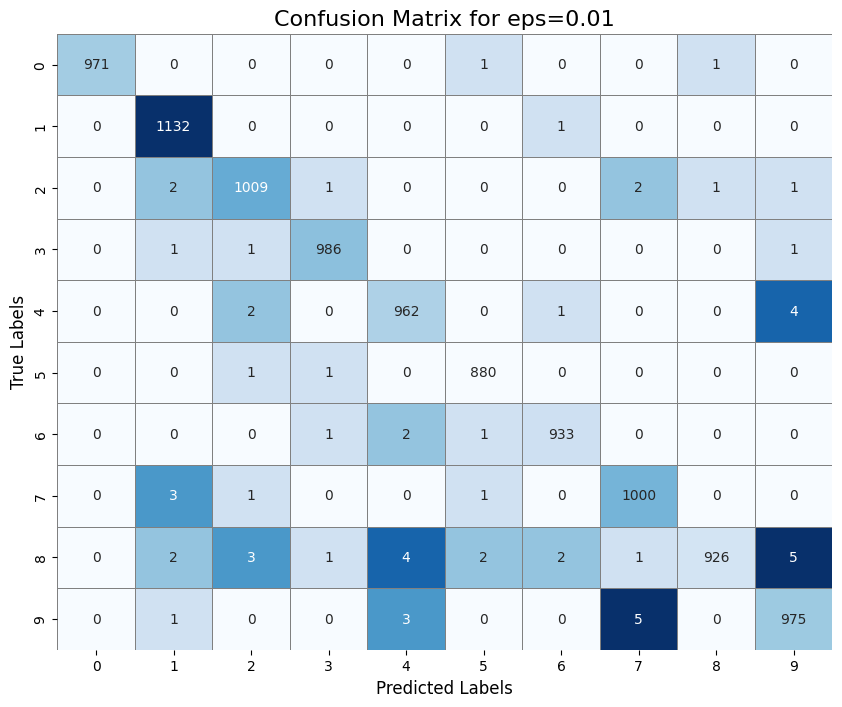
\includegraphics[width=\textwidth]{V2_images/_correct_labels_confusion_matrix_eps_0.01.png}
    \caption{confusion matrix 0.01 (output variable)}
    \label{fig:image1}
  \end{subfigure}
  \hfill
  \begin{subfigure}[b]{0.49\textwidth}
    \centering
    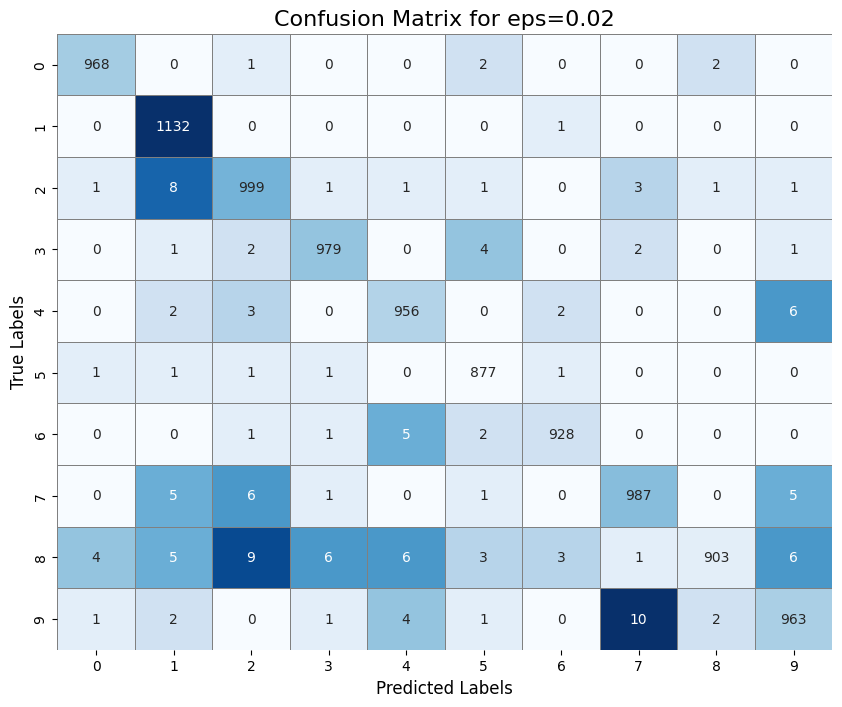
\includegraphics[width=\textwidth]{V2_images/_correct_labels_confusion_matrix_eps_0.02.png}
    \caption{confusion matrix 0.02 (output variable)}
    \label{fig:image2}
  \end{subfigure}

  \label{fig:images}
\end{figure*}

\begin{figure*}[h]
  \centering
  \begin{subfigure}[b]{0.49\textwidth}
    \centering
    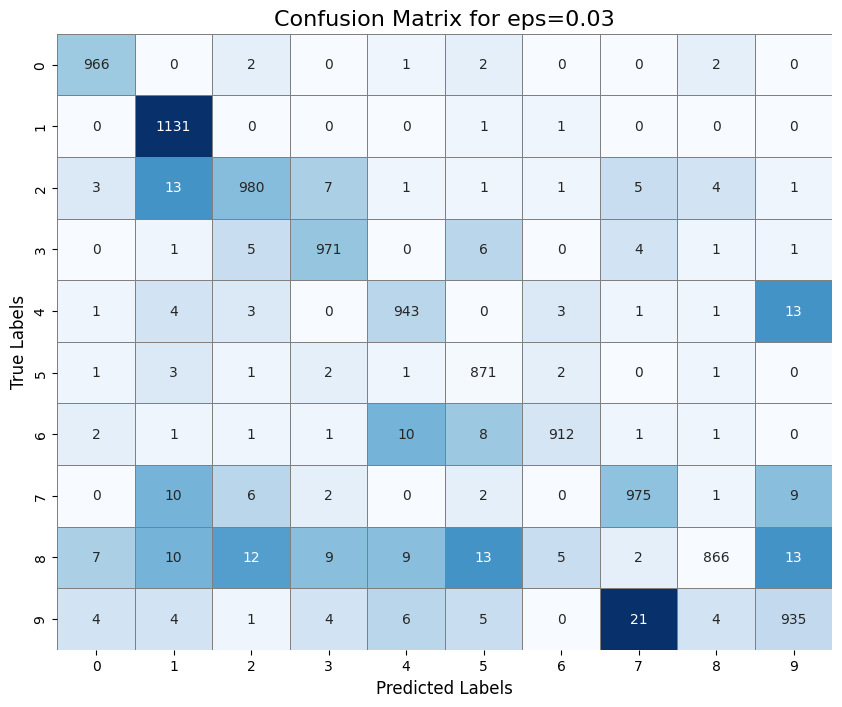
\includegraphics[width=\textwidth]{V2_images/_correct_labels_confusion_matrix_eps_0.03.png}
    \caption{confusion matrix 0.03 (output variable)}
    \label{fig:image1}
  \end{subfigure}
  \hfill
  \begin{subfigure}[b]{0.49\textwidth}
    \centering
    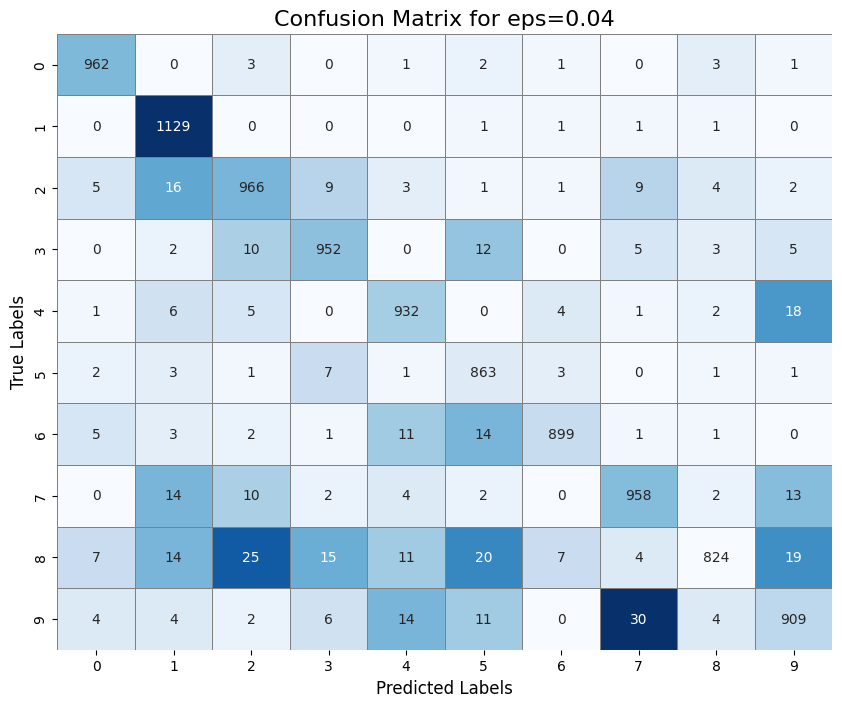
\includegraphics[width=\textwidth]{V2_images/_correct_labels_confusion_matrix_eps_0.04.png}
    \caption{confusion matrix 0.04 (output variable)}
    \label{fig:image2}
  \end{subfigure}

  \label{fig:images}
\end{figure*}

\begin{figure*}[h]
  \centering
  \begin{subfigure}[b]{0.49\textwidth}
    \centering
    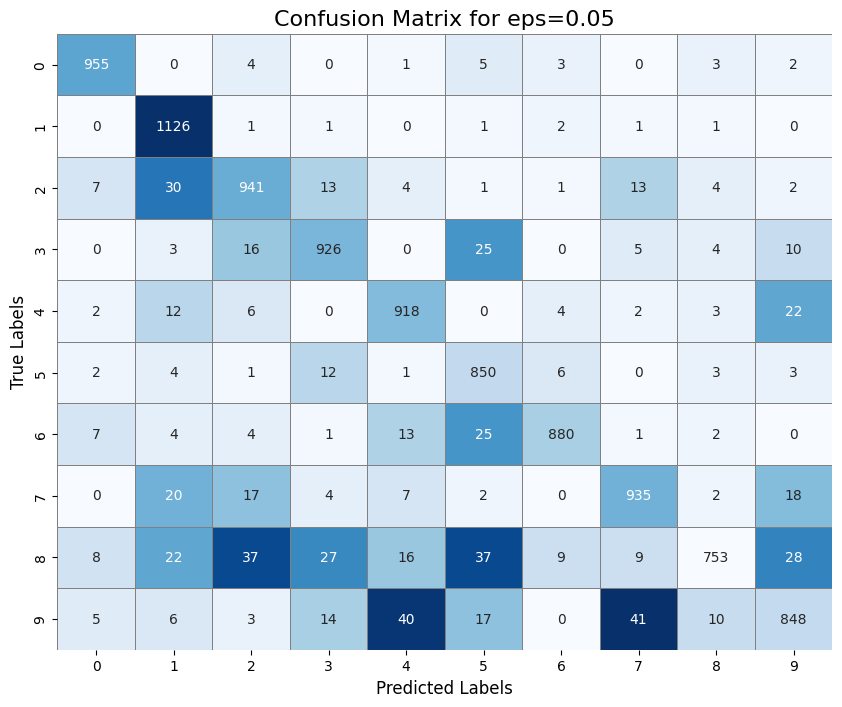
\includegraphics[width=\textwidth]{V2_images/_correct_labels_confusion_matrix_eps_0.05.png}
    \caption{confusion matrix 0.05 (output variable)}
    \label{fig:image1}
  \end{subfigure}
  \hfill
  \begin{subfigure}[b]{0.49\textwidth}
    \centering
    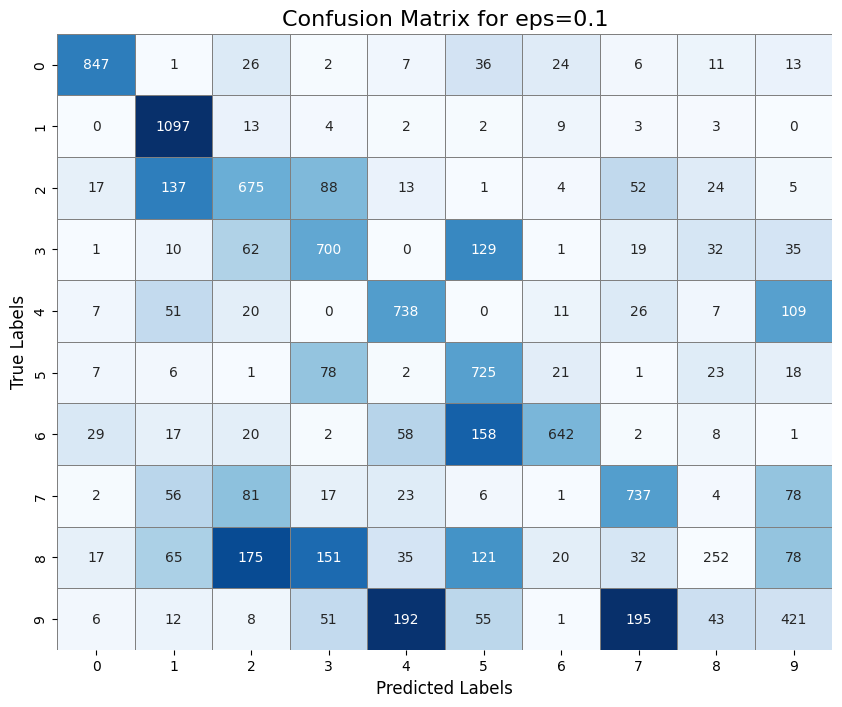
\includegraphics[width=\textwidth]{V2_images/_correct_labels_confusion_matrix_eps_0.1.png}
    \caption{confusion matrix 0.1 (output variable)}
    \label{fig:image2}
  \end{subfigure}

  \label{fig:images}
\end{figure*}

\begin{figure*}[h]
  \centering
  \begin{subfigure}[b]{0.49\textwidth}
    \centering
    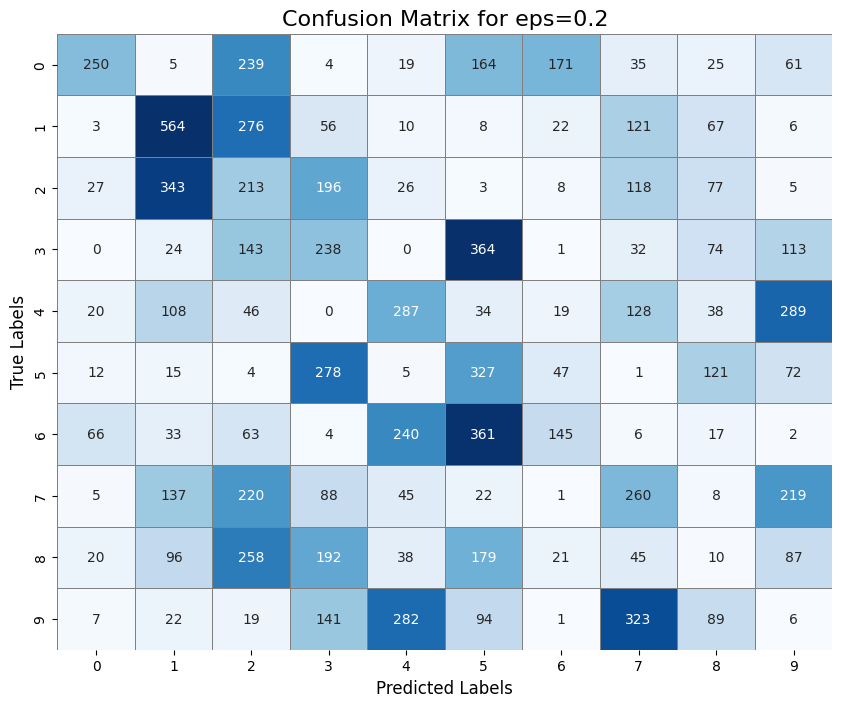
\includegraphics[width=\textwidth]{V2_images/_correct_labels_confusion_matrix_eps_0.2.png}
    \caption{confusion matrix 0.2(output variable)}
    \label{fig:image1}
  \end{subfigure}
  \hfill
  \begin{subfigure}[b]{0.49\textwidth}
    \centering
    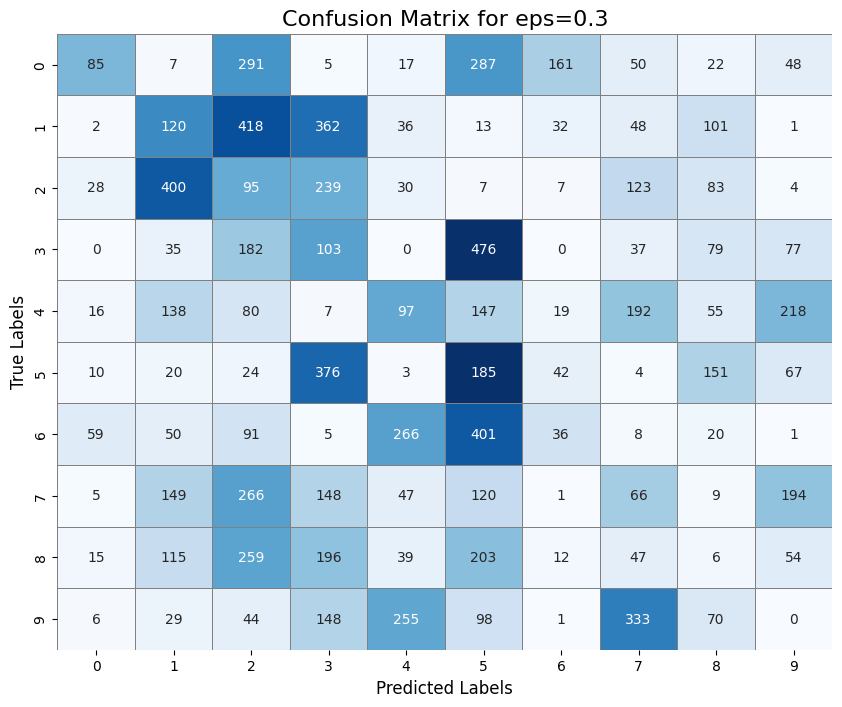
\includegraphics[width=\textwidth]{V2_images/_correct_labels_confusion_matrix_eps_0.3.png}
    \caption{confusion matrix 0.3 (output variable)}
    \label{fig:image2}
  \end{subfigure}
  \label{fig:images}
\end{figure*}

\begin{figure*}[h]
  \centering
  \begin{subfigure}[b]{0.49\textwidth}
    \centering
    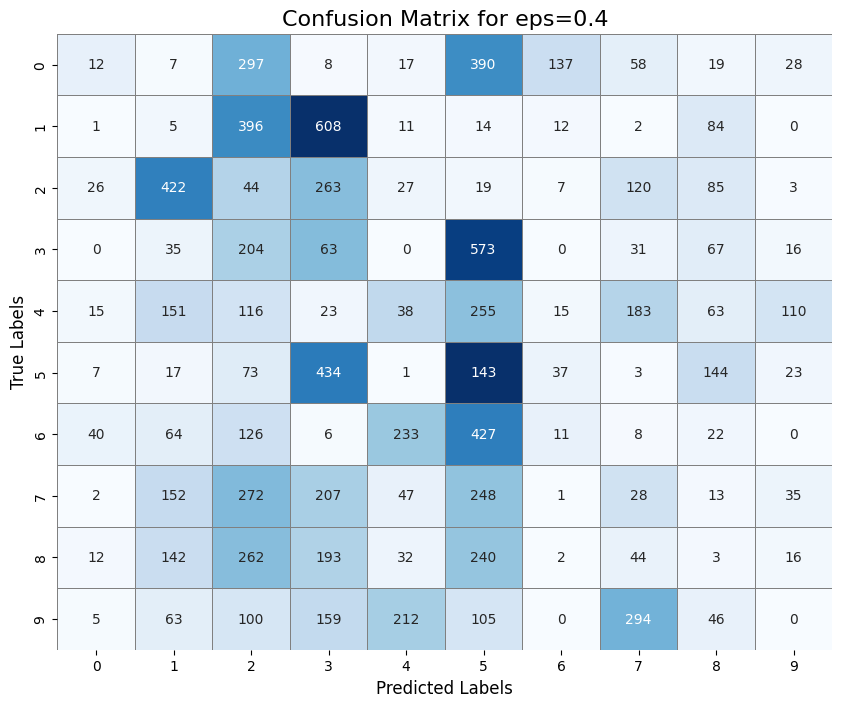
\includegraphics[width=\textwidth]{V2_images/_correct_labels_confusion_matrix_eps_0.4.png}
    \caption{confusion matrix 0.4 (output variable)}
    \label{fig:image1}
  \end{subfigure}
  \hfill
  \begin{subfigure}[b]{0.49\textwidth}
    \centering
    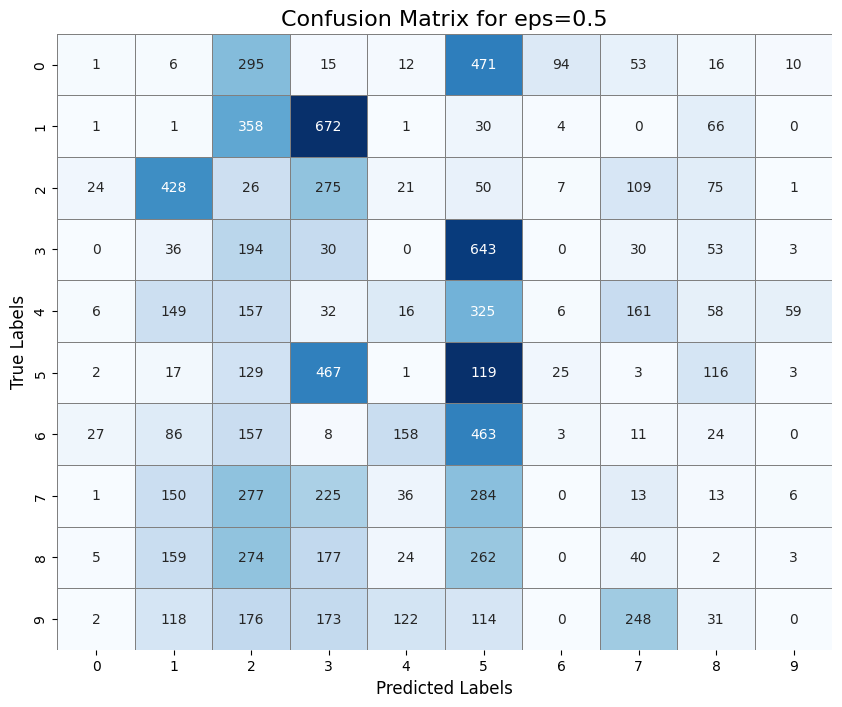
\includegraphics[width=\textwidth]{V2_images/_correct_labels_confusion_matrix_eps_0.5.png}
    \caption{confusion matrix 0.5 (output variable)}
    \label{fig:image2}
  \end{subfigure}
 
  \label{fig:images}
\end{figure*}

\begin{figure*}[h]
  \centering
  \begin{subfigure}[b]{0.49\textwidth}
    \centering
    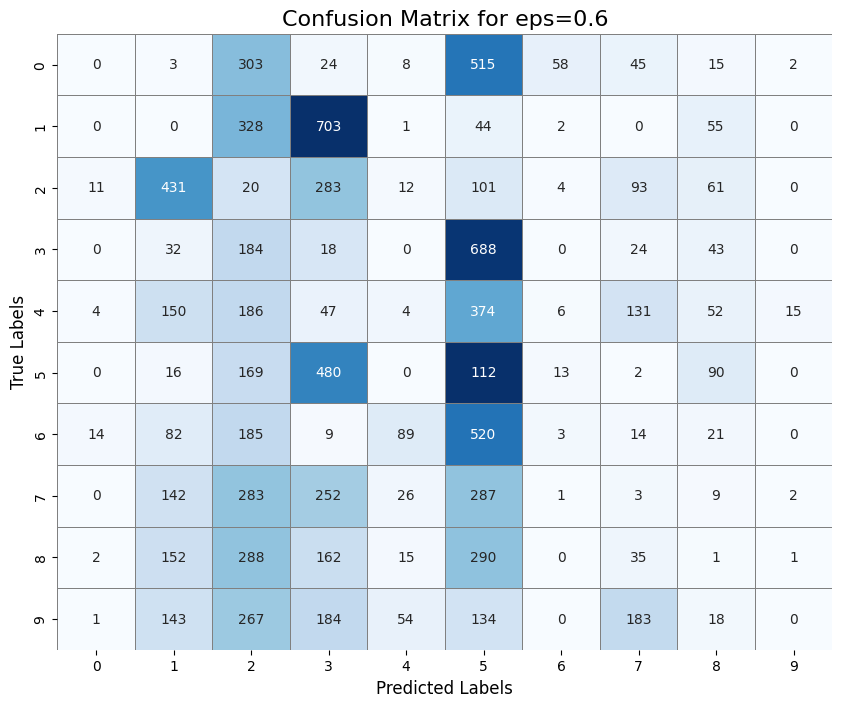
\includegraphics[width=\textwidth]{V2_images/_correct_labels_confusion_matrix_eps_0.6.png}
    \caption{confusion matrix 0.6 (output variable)}
    \label{fig:image1}
  \end{subfigure}
\end{figure*}

\clearpage % This will ensure that the title page is cleared before your sections start


\begin{table}[]
\footnotesize
\centering
\begin{tabular}{|l|l|l|l|l|}
\hline
            & \textbf{eps} & \textbf{num} & \textbf{with\_correct\_Labels}            & \textbf{without\_correct\_Labels} \\ \hline
\textbf{0}  & 0.01         & 1            & \{1: 9865\}                               & \{1: 9865\}              \\ \hline
\textbf{1}  & 0.01         & 2            & \{1: 9865\}                               & \{1: 9865\}              \\ \hline
\textbf{2}  & 0.01         & 3            & \{1: 9865\}                               & \{1: 9865\}              \\ \hline
\textbf{3}  & 0.01         & 4            & \{1: 9865\}                               & \{1: 9865\}              \\ \hline
\textbf{4}  & 0.01         & 5            & \{1: 9865\}                               & \{1: 9865\}              \\ \hline
\textbf{5}  & 0.02         & 1            & \{1: 9144, 5: 721\}                       & \{1: 4068, 5: 5797\}     \\ \hline
\textbf{6}  & 0.02         & 2            & \{1: 9144, 5: 721\}                       & \{1: 4068, 5: 5797\}     \\ \hline
\textbf{7}  & 0.02         & 3            & \{1: 9144, 5: 721\}                       & \{1: 4068, 5: 5797\}     \\ \hline
\textbf{8}  & 0.02         & 4            & \{1: 9144, 5: 721\}                       & \{1: 4068, 5: 5797\}     \\ \hline
\textbf{9}  & 0.02         & 5            & \{1: 9144, 5: 721\}                       & \{1: 4068, 5: 5797\}     \\ \hline
\textbf{10} & 0.03         & 1            & \{1: 8756, 5: 1109\}                      & \{1: 355, 5: 9510\}      \\ \hline
\textbf{11} & 0.03         & 2            & \{1: 8756, 5: 1109\}                      & \{1: 355, 5: 9510\}      \\ \hline
\textbf{12} & 0.03         & 3            & \{1: 8756, 5: 1109\}                      & \{1: 355, 5: 9510\}      \\ \hline
\textbf{13} & 0.03         & 4            & \{1: 8756, 5: 1109\}                      & \{1: 355, 5: 9510\}      \\ \hline
\textbf{14} & 0.03         & 5            & \{1: 8756, 5: 1109\}                      & \{1: 355, 5: 9510\}      \\ \hline
\textbf{15} & 0.04         & 1            & \{1: 8739, 5: 1126\}                      & \{1: 51, 5: 9813, 7: 1\} \\ \hline
\textbf{16} & 0.04         & 2            & \{1: 8739, 5: 1126\}                      & \{1: 51, 5: 9813, 7: 1\} \\ \hline
\textbf{17} & 0.04         & 3            & \{1: 8739, 5: 1126\}                      & \{1: 51, 5: 9813, 7: 1\} \\ \hline
\textbf{18} & 0.04         & 4            & \{1: 8739, 5: 1126\}                      & \{1: 51, 5: 9813, 7: 1\} \\ \hline
\textbf{19} & 0.04         & 5            & \{1: 8739, 5: 1126\}                      & \{1: 51, 5: 9813, 7: 1\} \\ \hline
\textbf{20} & 0.05         & 1            & \{1: 8735, 5: 1130\}                      & \{1: 12, 5: 9853\}       \\ \hline
\textbf{21} & 0.05         & 2            & \{1: 8735, 5: 1130\}                      & \{1: 12, 5: 9853\}       \\ \hline
\textbf{22} & 0.05         & 3            & \{1: 8735, 5: 1130\}                      & \{1: 12, 5: 9853\}       \\ \hline
\textbf{23} & 0.05         & 4            & \{1: 8735, 5: 1130\}                      & \{1: 12, 5: 9853\}       \\ \hline
\textbf{24} & 0.05         & 5            & \{1: 8735, 5: 1130\}                      & \{1: 12, 5: 9853\}       \\ \hline
\textbf{25} & 0.10         & 1            & \{1: 8512, 5: 1353\}                      & \{1: 1, 5: 9863, 7: 1\}  \\ \hline
\textbf{26} & 0.10         & 2            & \{1: 8512, 5: 1353\}                      & \{1: 1, 5: 9863, 7: 1\}  \\ \hline
\textbf{27} & 0.10         & 3            & \{1: 8512, 5: 1353\}                      & \{1: 1, 5: 9863, 7: 1\}  \\ \hline
\textbf{28} & 0.10         & 4            & \{1: 8512, 5: 1353\}                      & \{1: 1, 5: 9863, 7: 1\}  \\ \hline
\textbf{29} & 0.10         & 5            & \{1: 8512, 5: 1353\}                      & \{1: 1, 5: 9863, 7: 1\}  \\ \hline
\textbf{30} & 0.20         & 1            & \{1: 6911, 5: 2954\}                      & \{5: 9865\}              \\ \hline
\textbf{31} & 0.20         & 2            & \{1: 6911, 5: 2954\}                      & \{5: 9865\}              \\ \hline
\textbf{32} & 0.20         & 3            & \{1: 6911, 5: 2954\}                      & \{5: 9865\}              \\ \hline
\textbf{33} & 0.20         & 4            & \{1: 6911, 5: 2954\}                      & \{5: 9865\}              \\ \hline
\textbf{34} & 0.20         & 5            & \{1: 6911, 5: 2954\}                      & \{5: 9865\}              \\ \hline
\textbf{35} & 0.30         & 1            & \{1: 5219, 2: 45, 3: 6, 5: 4593, 7: 2\}   & \{5: 9865\}              \\ \hline
\textbf{36} & 0.30         & 2            & \{1: 5219, 2: 45, 3: 6, 5: 4593, 7: 2\}   & \{5: 9865\}              \\ \hline
\textbf{37} & 0.30         & 3            & \{1: 5219, 2: 45, 3: 6, 5: 4593, 7: 2\}   & \{5: 9865\}              \\ \hline
\textbf{38} & 0.30         & 4            & \{1: 5219, 2: 45, 3: 6, 5: 4593, 7: 2\}   & \{5: 9865\}              \\ \hline
\textbf{39} & 0.30         & 5            & \{1: 5219, 2: 45, 3: 6, 5: 4593, 7: 2\}   & \{5: 9865\}              \\ \hline
\textbf{40} & 0.40         & 1            & \{1: 3701, 2: 192, 3: 10, 5: 5958, 7: 4\} & \{5: 9865\}              \\ \hline
\textbf{41} & 0.40         & 2            & \{1: 3701, 2: 192, 3: 10, 5: 5958, 7: 4\} & \{5: 9865\}              \\ \hline
\textbf{42} & 0.40         & 3            & \{1: 3701, 2: 192, 3: 10, 5: 5958, 7: 4\} & \{5: 9865\}              \\ \hline
\textbf{43} & 0.40         & 4            & \{1: 3701, 2: 192, 3: 10, 5: 5958, 7: 4\} & \{5: 9865\}              \\ \hline
\textbf{44} & 0.40         & 5            & \{1: 3701, 2: 192, 3: 10, 5: 5958, 7: 4\} & \{5: 9865\}              \\ \hline
\textbf{45} & 0.50         & 1            & \{1: 2522, 2: 342, 3: 20, 5: 6977, 7: 4\} & \{5: 9865\}              \\ \hline
\textbf{46} & 0.50         & 2            & \{1: 2522, 2: 342, 3: 20, 5: 6977, 7: 4\} & \{5: 9865\}              \\ \hline
\textbf{47} & 0.50         & 3            & \{1: 2522, 2: 342, 3: 20, 5: 6977, 7: 4\} & \{5: 9865\}              \\ \hline
\textbf{48} & 0.50         & 4            & \{1: 2522, 2: 342, 3: 20, 5: 6977, 7: 4\} & \{5: 9865\}              \\ \hline
\textbf{49} & 0.50         & 5            & \{1: 2522, 2: 342, 3: 20, 5: 6977, 7: 4\} & \{5: 9865\}              \\ \hline
\textbf{50} & 0.60         & 1            & \{1: 1675, 2: 472, 3: 45, 5: 7670, 7: 3\} & \{5: 9865\}              \\ \hline
\textbf{51} & 0.60         & 2            & \{1: 1675, 2: 472, 3: 45, 5: 7670, 7: 3\} & \{5: 9865\}              \\ \hline
\textbf{52} & 0.60         & 3            & \{1: 1675, 2: 472, 3: 45, 5: 7670, 7: 3\} & \{5: 9865\}              \\ \hline
\textbf{53} & 0.60         & 4            & \{1: 1675, 2: 472, 3: 45, 5: 7670, 7: 3\} & \{5: 9865\}              \\ \hline
\textbf{54} & 0.60         & 5            & \{1: 1675, 2: 472, 3: 45, 5: 7670, 7: 3\} & \{5: 9865\}              \\ \hline
\end{tabular}
\end{table}
\clearpage % This will ensure that the title page is cleared before your sections start

\section{Multiple Attacks Without True Labels}

\begin{algorithm}[H]
\caption{Adversarial Attack Evaluation}
\begin{algorithmic}[1]
\State $\text{eps\_range} \gets [0.01, 0.02, 0.03, \ldots, 0.6]$
\State $\text{results\_df} \gets \text{DataFrame()}$
\For{$\text{eps} \in \text{eps\_range}$}
    \For{$\text{attack\_num} \gets 1 \text{ to } 5$}
        \State $\text{attack} \gets \text{FastGradientMethod}(\text{classifier}, \text{eps})$
        \State $\text{x\_adv} \gets \text{attack.generate}(\text{x=correct\_examples})$
        \State $\text{y\_adv} \gets \text{classifier.predict}(\text{x\_adv})$
        \State $\text{cm} \gets \text{confusion\_matrix}(\text{correct\_labels}, \text{y\_adv})$
        \State $\text{Save heatmap of cm to file}$
        \State $\text{results\_df.append}(\{\text{'eps'}: \text{eps}, \text{'attack\_num'}: \text{attack\_num}, \ldots\})$
    \EndFor
\EndFor
\State $\text{results\_df.to\_csv}(\text{'/content/drive/MyDrive/ColabNotebooks/adv\_results.csv'})$
\State $\text{Print}(\text{results\_df})$
\end{algorithmic}
\end{algorithm}

\begin{figure*}[h]
  \centering
  \begin{subfigure}[b]{0.49\textwidth}
    \centering
    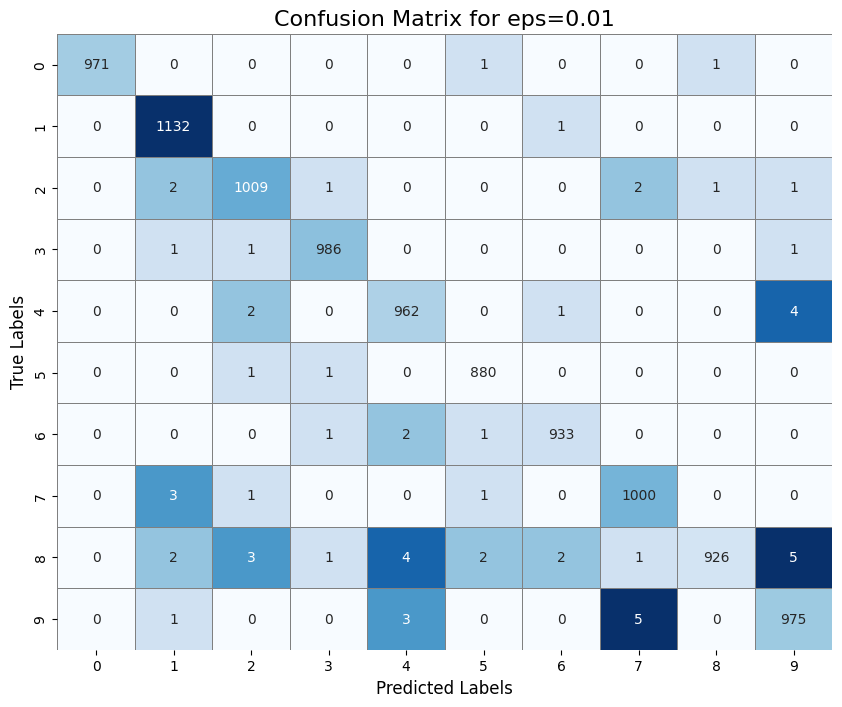
\includegraphics[width=\textwidth]{V2_images/confusion_matrix_eps_0.01_attack_1.png}
    \caption{confusion matrix 0.01 attack1}
    \label{fig:image1}
  \end{subfigure}
  \hfill
  \begin{subfigure}[b]{0.49\textwidth}
    \centering
    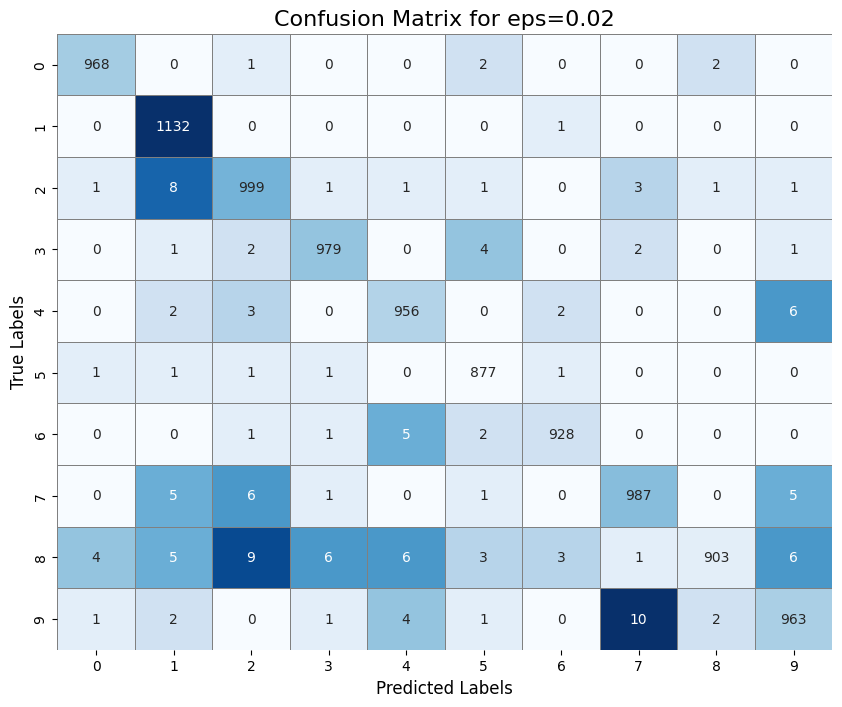
\includegraphics[width=\textwidth]{V2_images/confusion_matrix_eps_0.02_attack_1.png}
    \caption{confusion matrix 0.02 attack1}
    \label{fig:image2}
  \end{subfigure}
  
  \label{fig:images}
\end{figure*}

\begin{figure*}[h]
  \centering
  \begin{subfigure}[b]{0.49\textwidth}
    \centering
    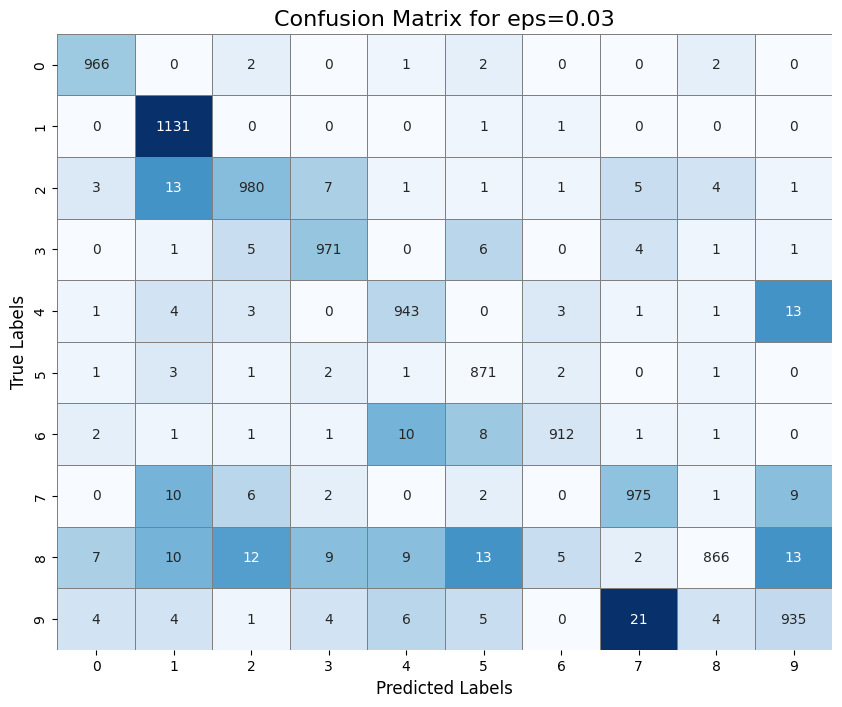
\includegraphics[width=\textwidth]{V2_images/confusion_matrix_eps_0.03_attack_1.png}
    \caption{confusion matrix 0.03 attack1}
    \label{fig:image1}
  \end{subfigure}
  \hfill
  \begin{subfigure}[b]{0.49\textwidth}
    \centering
    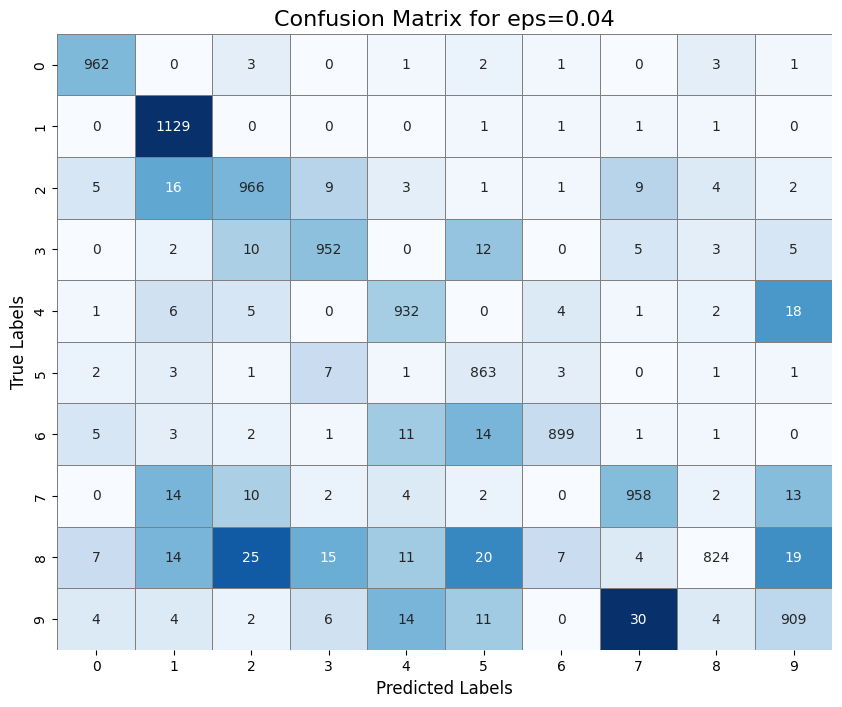
\includegraphics[width=\textwidth]{V2_images/confusion_matrix_eps_0.04_attack_1.png}
    \caption{confusion matrix 0.04 attack1}
    \label{fig:image2}
  \end{subfigure}
  \label{fig:images}
\end{figure*}


\begin{figure*}[h]
  \centering
  \begin{subfigure}[b]{0.49\textwidth}
    \centering
    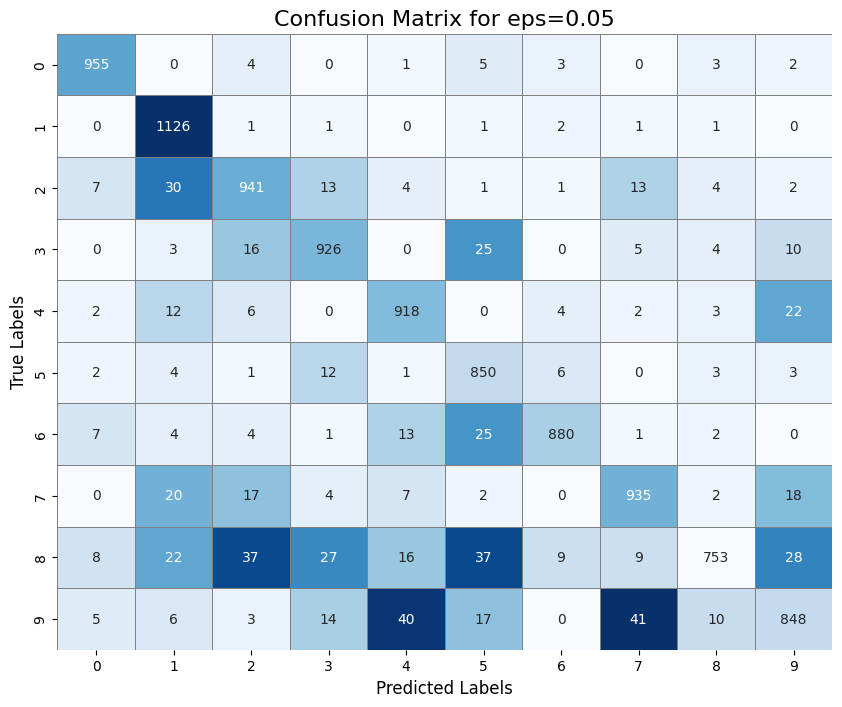
\includegraphics[width=\textwidth]{V2_images/confusion_matrix_eps_0.05_attack_1.png}
    \caption{confusion matrix 0.05 attack1}
    \label{fig:image1}
  \end{subfigure}
  \hfill
  \begin{subfigure}[b]{0.49\textwidth}
    \centering
    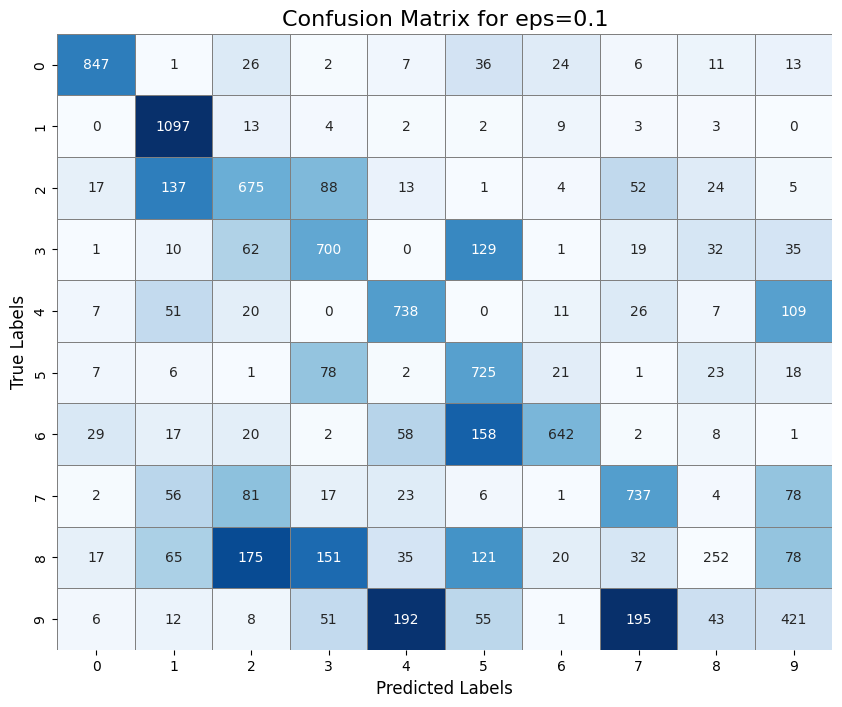
\includegraphics[width=\textwidth]{V2_images/confusion_matrix_eps_0.1_attack_1.png}
    \caption{confusion matrix 0.1 attack1}
    \label{fig:image2}
  \end{subfigure}
  \label{fig:images}
\end{figure*}


\begin{figure*}[h]
  \centering
  \begin{subfigure}[b]{0.49\textwidth}
    \centering
    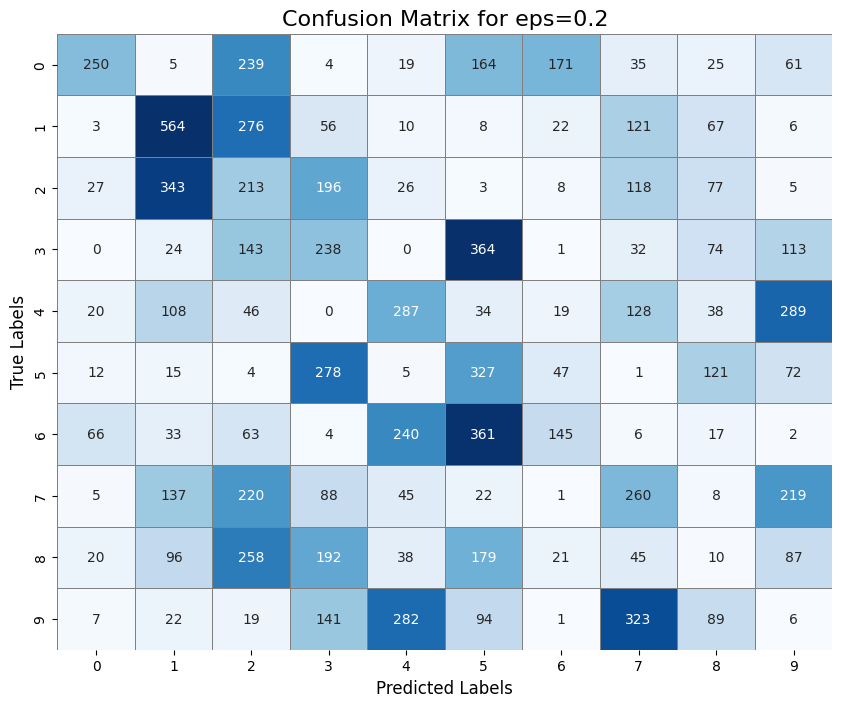
\includegraphics[width=\textwidth]{V2_images/confusion_matrix_eps_0.2_attack_1.png}
    \caption{confusion matrix 0.2 attack1}
    \label{fig:image1}
  \end{subfigure}
  \hfill
  \begin{subfigure}[b]{0.49\textwidth}
    \centering
    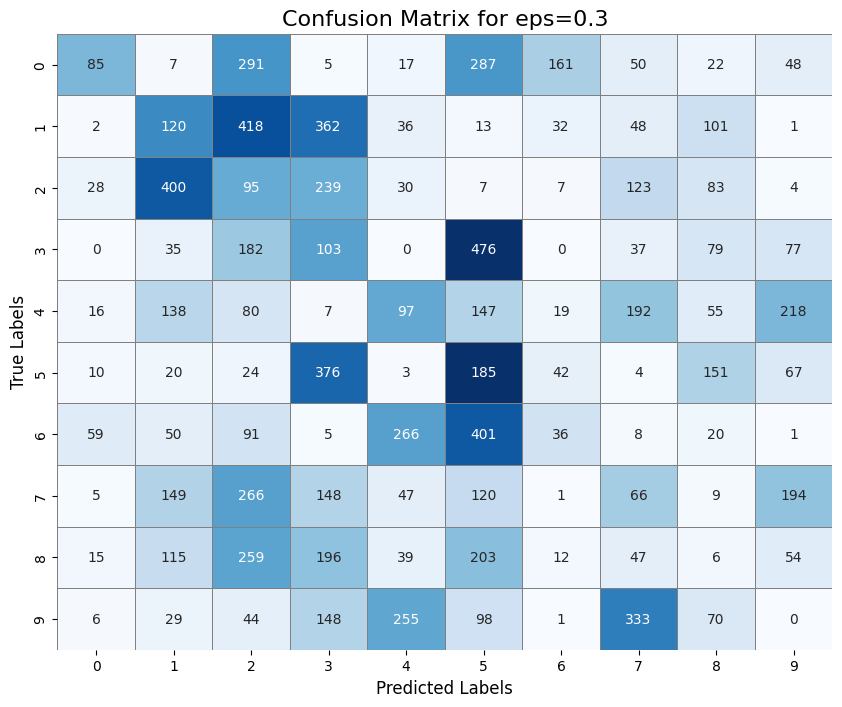
\includegraphics[width=\textwidth]{V2_images/confusion_matrix_eps_0.3_attack_1.png}
    \caption{confusion matrix 0.3 attack1}
    \label{fig:image2}
  \end{subfigure}
  \label{fig:images}
\end{figure*}


\begin{figure*}[h]
  \centering
  \begin{subfigure}[b]{0.49\textwidth}
    \centering
    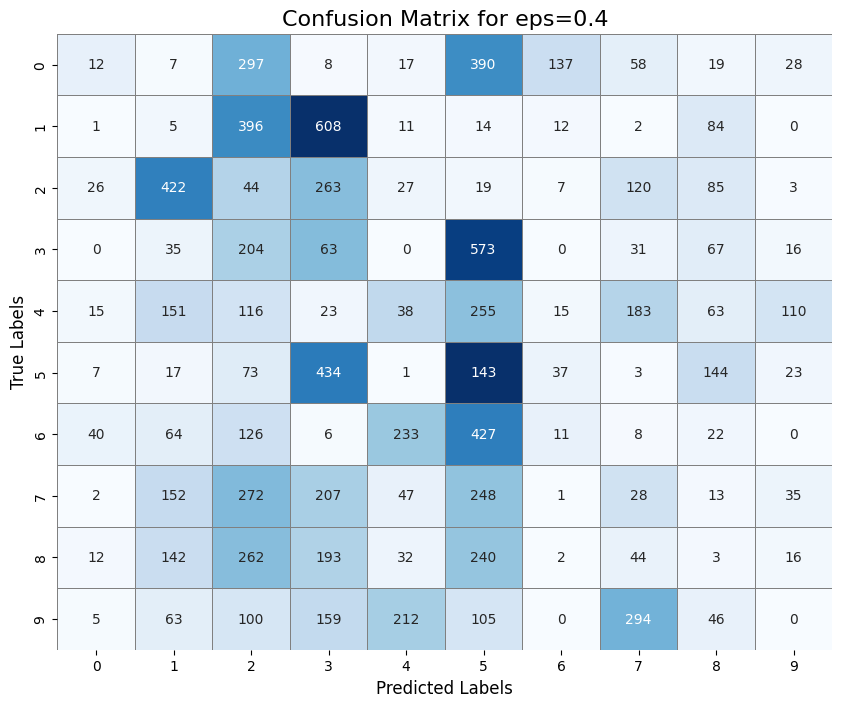
\includegraphics[width=\textwidth]{V2_images/confusion_matrix_eps_0.4_attack_1.png}
    \caption{confusion matrix 0.4 attack1}
    \label{fig:image1}
  \end{subfigure}
  \hfill
  \begin{subfigure}[b]{0.49\textwidth}
    \centering
    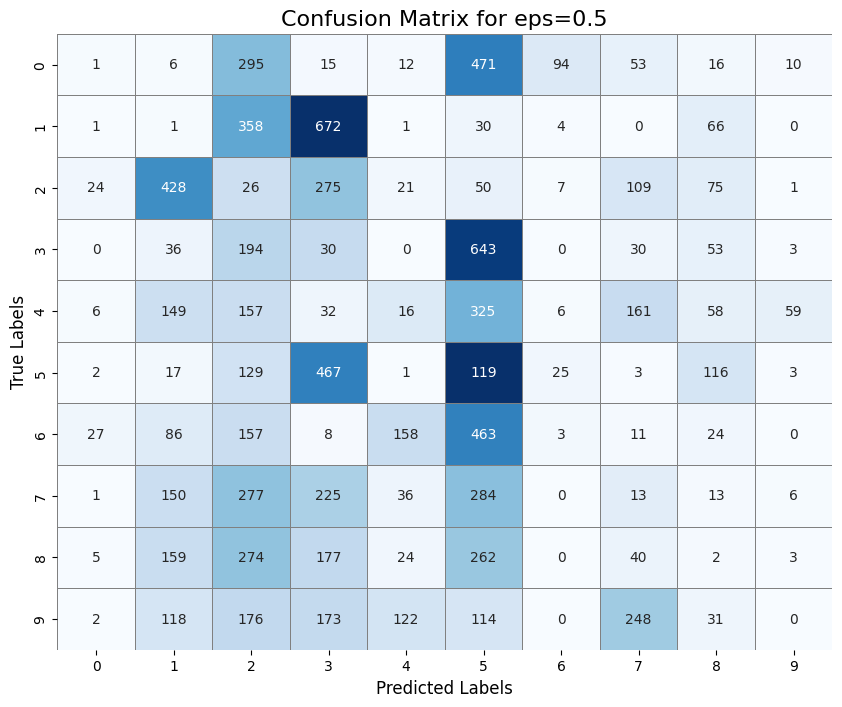
\includegraphics[width=\textwidth]{V2_images/confusion_matrix_eps_0.5_attack_1.png}
    \caption{confusion matrix 0.5 attack1}
    \label{fig:image2}
  \end{subfigure}
  \label{fig:images}
\end{figure*}


\begin{figure*}[h]
  \centering
  \begin{subfigure}[b]{0.49\textwidth}
    \centering
    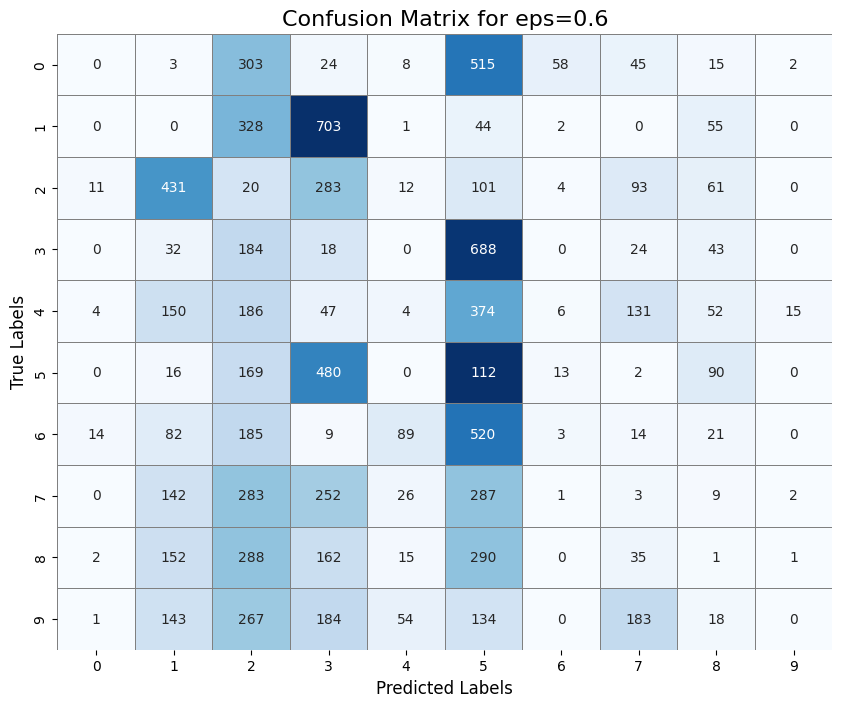
\includegraphics[width=\textwidth]{V2_images/confusion_matrix_eps_0.6_attack_1.png}
    \caption{confusion matrix 0.6 attack1}
    \label{fig:image1}
  \end{subfigure}
  
\end{figure*}
%%

\clearpage % This will ensure that the title page is cleared before your sections start

\section{Multiple Attacks With True Labels}
\begin{algorithm}[H]
\caption{Adversarial Attack Evaluation}
\begin{algorithmic}[1]
\State $\text{eps\_range} \gets [0.01, 0.02, 0.03, \ldots, 0.6]$
\State $\text{results\_df} \gets \text{DataFrame()}$
\For{$\text{eps} \in \text{eps\_range}$}
    \For{$\text{attack\_num} \gets 1 \text{ to } 5$}
        \State $\text{attack} \gets \text{FastGradientMethod}(\text{classifier}, \text{eps})$
        \State $\text{x\_adv} \gets \text{attack.generate}(\text{x=correct\_examples,y=correct\_labels})$
        \State $\text{y\_adv} \gets \text{classifier.predict}(\text{x\_adv})$
        \State $\text{cm} \gets \text{confusion\_matrix}(\text{correct\_labels}, \text{y\_adv})$
        \State $\text{Save heatmap of cm to file}$
        \State $\text{results\_df.append}(\{\text{'eps'}: \text{eps}, \text{'attack\_num'}: \text{attack\_num}, \ldots\})$
    \EndFor
\EndFor
\State $\text{results\_df.to\_csv}(\text{'/content/drive/MyDrive/ColabNotebooks/adv\_results.csv'})$
\State $\text{Print}(\text{results\_df})$
\end{algorithmic}
\end{algorithm}
%%%%%%%%%%%%%%%%%%%%%%%%%%%%%%%%%%%\
\begin{figure*}[h]
  \centering
  \begin{subfigure}[b]{0.49\textwidth}
    \centering
    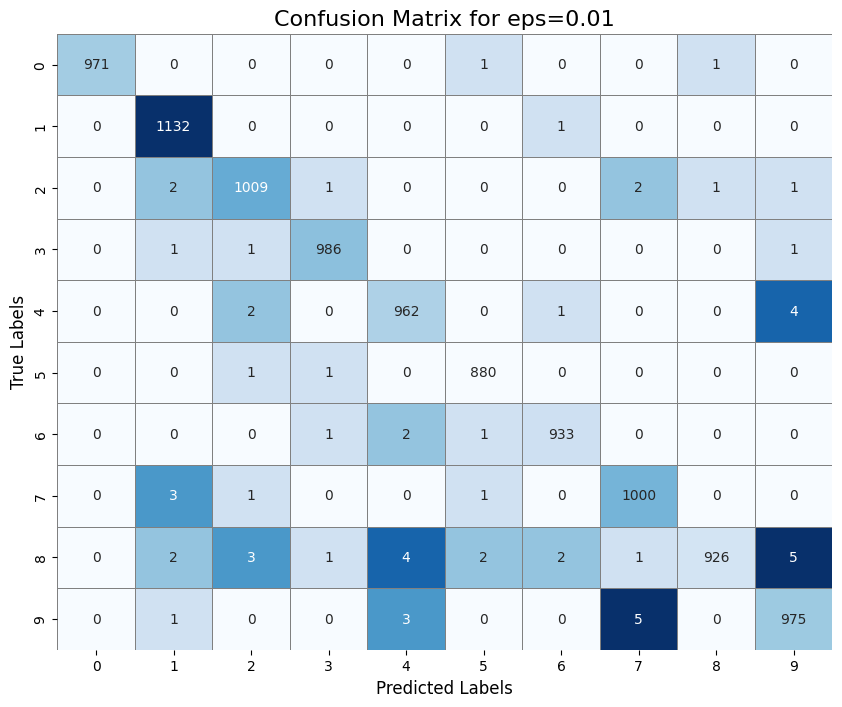
\includegraphics[width=\textwidth]{V2_images/target_confusion_matrix_eps_0.01_attack_1.png}
    \caption{confusion matrix 0.01}
    \label{fig:image1}
  \end{subfigure}
  \hfill
  \begin{subfigure}[b]{0.49\textwidth}
    \centering
    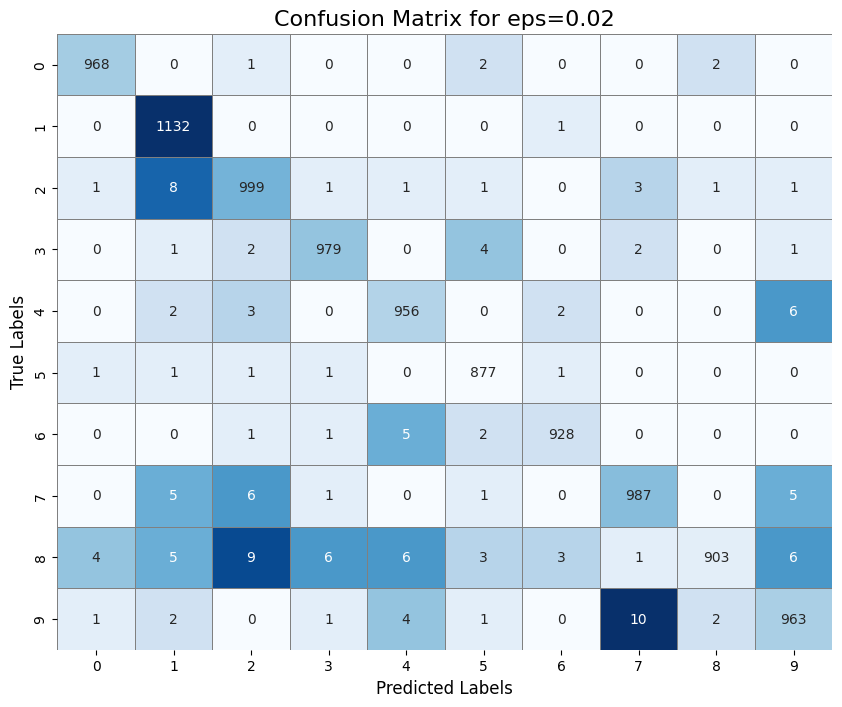
\includegraphics[width=\textwidth]{V2_images/target_confusion_matrix_eps_0.02_attack_1.png}
    \caption{confusion matrix 0.02}
    \label{fig:image2}
  \end{subfigure}
  
  \label{fig:images}
\end{figure*}

\begin{figure*}[h]
  \centering
  \begin{subfigure}[b]{0.49\textwidth}
    \centering
    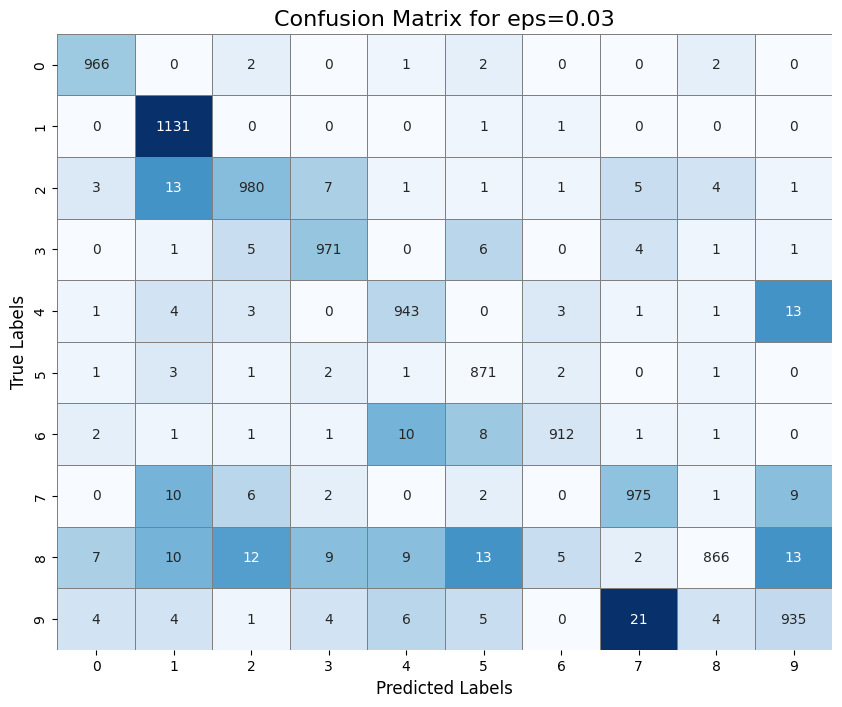
\includegraphics[width=\textwidth]{V2_images/target_confusion_matrix_eps_0.03_attack_1.png}
    \caption{confusion matrix 0.03}
    \label{fig:image1}
  \end{subfigure}
  \hfill
  \begin{subfigure}[b]{0.49\textwidth}
    \centering
    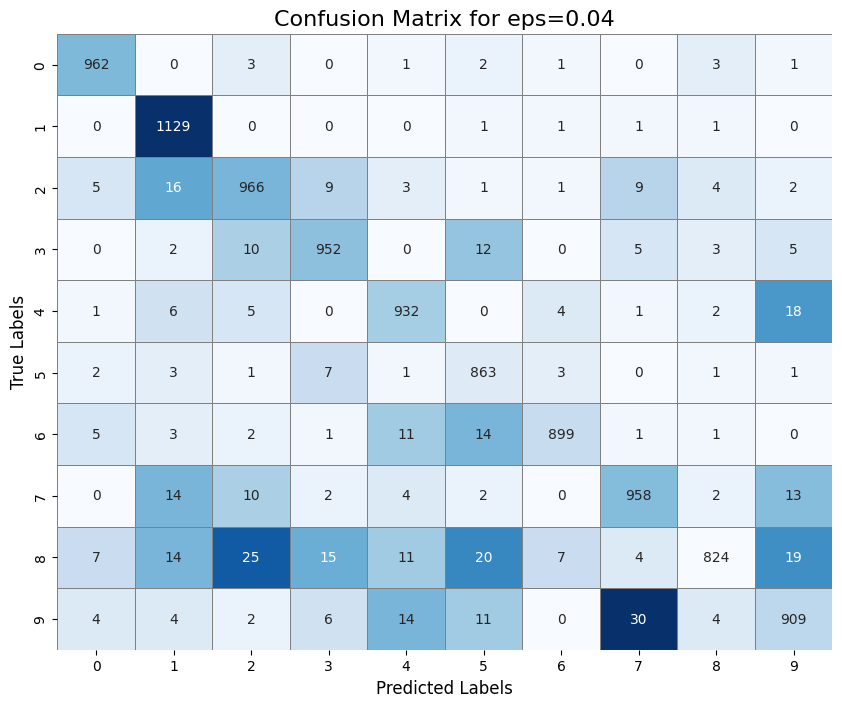
\includegraphics[width=\textwidth]{V2_images/target_confusion_matrix_eps_0.04_attack_1.png}
    \caption{confusion matrix 0.04}
    \label{fig:image2}
  \end{subfigure}
 
  \label{fig:images}
\end{figure*}


\begin{figure*}[h]
  \centering
  \begin{subfigure}[b]{0.49\textwidth}
    \centering
    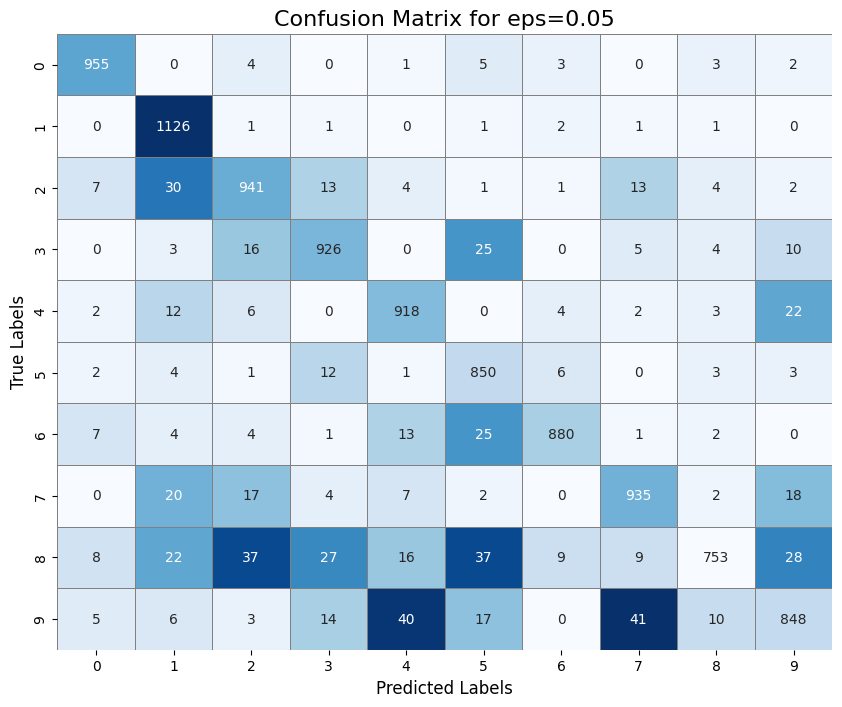
\includegraphics[width=\textwidth]{V2_images/target_confusion_matrix_eps_0.05_attack_1.png}
    \caption{confusion matrix 0.05}
    \label{fig:image1}
  \end{subfigure}
  \hfill
  \begin{subfigure}[b]{0.49\textwidth}
    \centering
    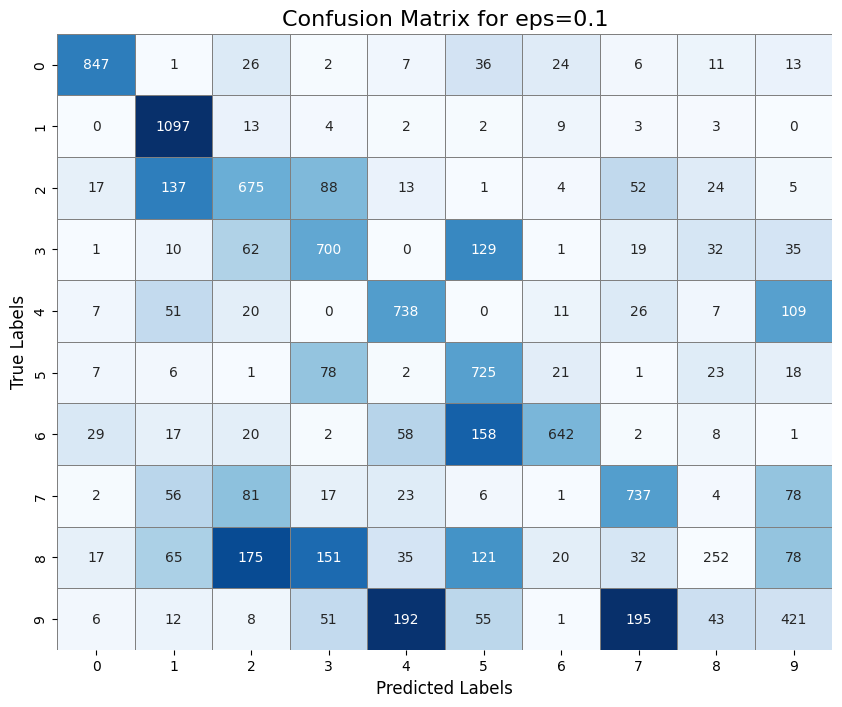
\includegraphics[width=\textwidth]{V2_images/target_confusion_matrix_eps_0.1_attack_1.png}
    \caption{confusion matrix 0.1}
    \label{fig:image2}
  \end{subfigure}
  \label{fig:images}
\end{figure*}


\begin{figure*}[h]
  \centering
  \begin{subfigure}[b]{0.49\textwidth}
    \centering
    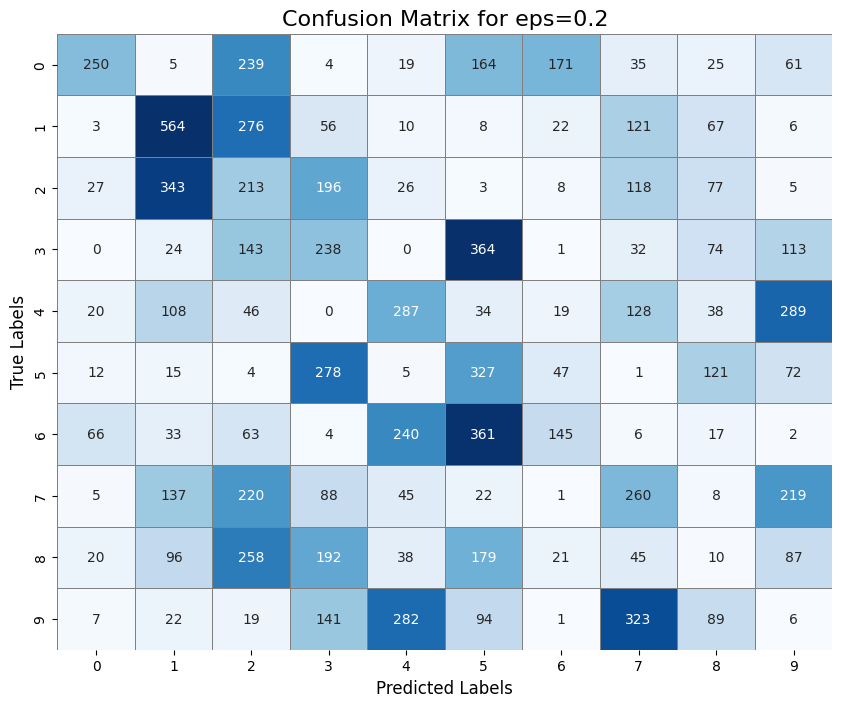
\includegraphics[width=\textwidth]{V2_images/target_confusion_matrix_eps_0.2_attack_1.png}
    \caption{confusion matrix 0.2}
    \label{fig:image1}
  \end{subfigure}
  \hfill
  \begin{subfigure}[b]{0.49\textwidth}
    \centering
    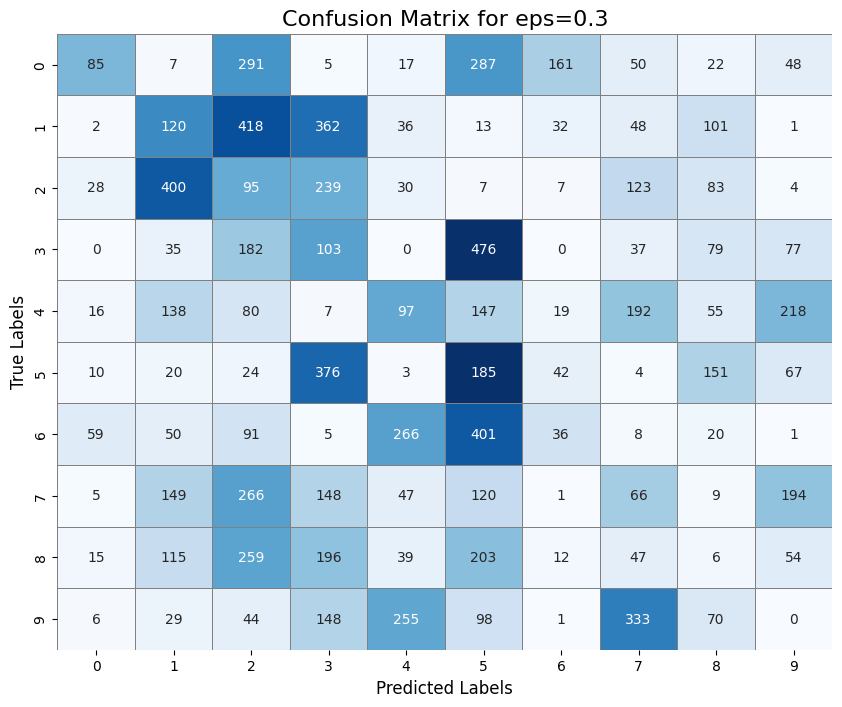
\includegraphics[width=\textwidth]{V2_images/target_confusion_matrix_eps_0.3_attack_1.png}
    \caption{confusion matrix 0.3}
    \label{fig:image2}
  \end{subfigure}

\end{figure*}


\begin{figure*}[h]
  \centering
  \begin{subfigure}[b]{0.49\textwidth}
    \centering
    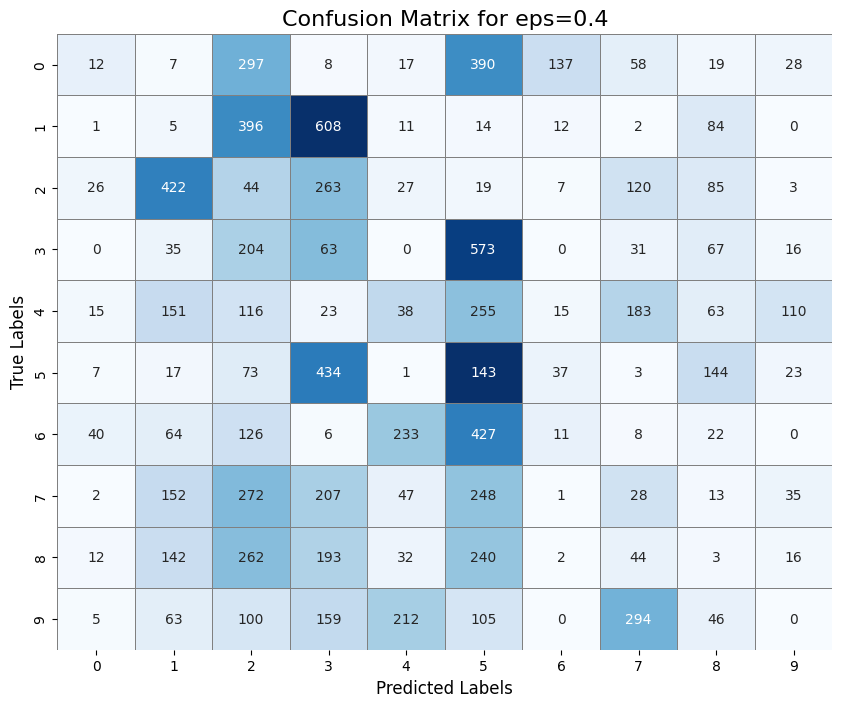
\includegraphics[width=\textwidth]{V2_images/target_confusion_matrix_eps_0.4_attack_1.png}
    \caption{confusion matrix 0.4 }
    \label{fig:image1}
  \end{subfigure}
  \hfill
  \begin{subfigure}[b]{0.49\textwidth}
    \centering
    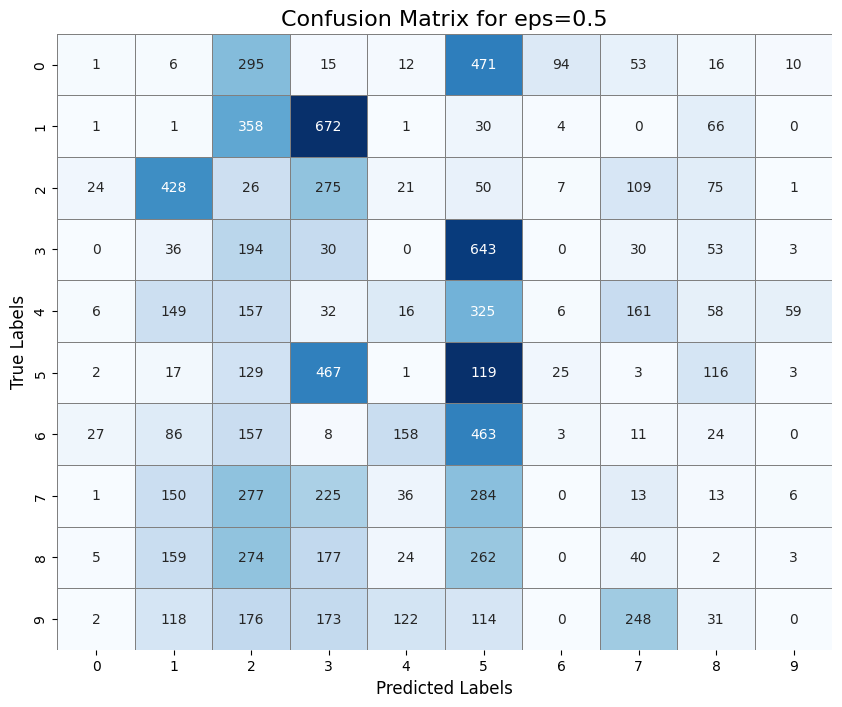
\includegraphics[width=\textwidth]{V2_images/target_confusion_matrix_eps_0.5_attack_1.png}
    \caption{confusion matrix 0.5 }
    \label{fig:image2}
  \end{subfigure}
  
  \label{fig:images}
\end{figure*}


\begin{figure*}[h]
  \centering
  \begin{subfigure}[b]{0.49\textwidth}
    \centering
    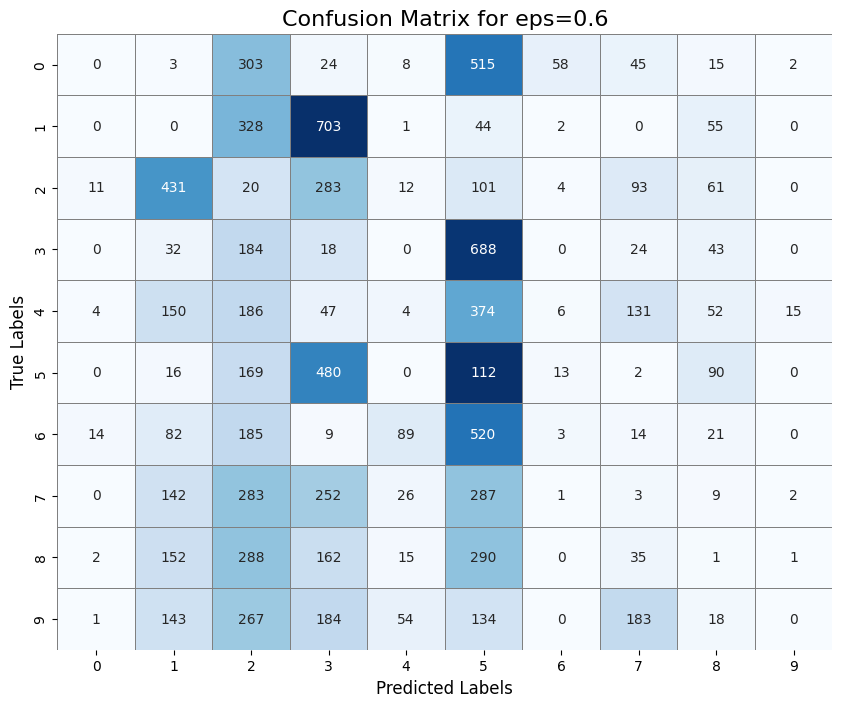
\includegraphics[width=\textwidth]{V2_images/target_confusion_matrix_eps_0.6_attack_1.png}
    \caption{confusion matrix 0.6 }
    \label{fig:image1}
  \end{subfigure}
  
\end{figure*}

\end{document}
